% main.tex  —  TMR4115 Design Methods Compendium
% Build:  latexmk -pdf -outdir=build main.tex
% =====================================================================
\documentclass[11pt,a4paper]{book}

\usepackage[T1]{fontenc}          % proper hyphenation of accented words
\usepackage{lmodern}
\usepackage{amsmath,amssymb}      % maths
\usepackage{booktabs}             % \toprule \midrule \bottomrule
\usepackage{graphicx}             % \includegraphics
\usepackage{float}                % [H] float placement
\usepackage{tikz}                 % diagrams drawn in the text
\usetikzlibrary{arrows.meta,positioning}
\usepackage{listings}             % Python code listings
\usepackage[authoryear,round]{natbib}
\usepackage[hidelinks]{hyperref}  % load last

% Figures live in fig/<chapter>/, referenced as {ch_name/file.png}
\graphicspath{{fig/}}

\lstset{
  basicstyle=\ttfamily\footnotesize,
  breaklines=true,
  frame=single,
  columns=fullflexible,
  keywordstyle=\color{blue!60!black},
  commentstyle=\color{gray}
}

% =====================================================================
\begin{document}

\frontmatter
\tableofcontents

\mainmatter

% % ch_ship_size_speed.tex  —  stub
% Replace this with chapter content

% % ch_configuration.tex  —  stub
% Replace this with chapter content

% ch_lp_types.tex  —  Chapter: Linear programming: formulation and application to ship configuration design
% Content only — compiled via main.tex
% Figures in fig/, code in code/
\chapter{Linear programming: formulation and application to ship configuration design}
\label{ch:lp-intro}

In the previous chapter, ship size and speed were treated as continuous
production factors, and the optimal combination followed from setting a
derivative to zero. Most design decisions are not that unconstrained: a
designer choosing how much cargo to load, how many cabins of each type to
build, or how to lay out equipment on a deck is working against explicit
limits on weight, area, length, or capacity. \emph{Linear programming} (LP)
is the natural first tool for this class of problem: it handles many
decision variables and many constraints simultaneously, as long as the
objective and the constraints are linear in the decision variables.

This chapter introduces the structure of a linear program, develops a
disciplined approach to formulating design problems mathematically, and
applies both to a recurring class of ship design problem: allocating a
scarce resource (deck area, side length, tank volume) across a set of
competing uses. The cabin arrangement problem, used throughout, is a small
but genuine instance of what is generally called a \emph{general
arrangement} or \emph{configuration} problem.

\section{The structure of a linear program}

\subsection{Decision variables, objective function, and constraints}

A linear program has three ingredients: a set of \emph{decision variables}
$x_1, x_2, \ldots, x_n$ representing quantities the designer controls; a
linear \emph{objective function} to be maximized or minimized; and a set of
linear \emph{constraints} that the variables must satisfy. In maximization
form,
\begin{align}
  \max \quad & Z = c_1 x_1 + c_2 x_2 + \cdots + c_n x_n \label{eq:lp-obj}\\
  \text{s.t.} \quad & a_{11}x_1 + a_{12}x_2 + \cdots + a_{1n}x_n \leq b_1 \notag\\
  & \qquad\qquad \vdots \notag\\
  & a_{m1}x_1 + a_{m2}x_2 + \cdots + a_{mn}x_n \leq b_m \notag\\
  & x_1, x_2, \ldots, x_n \geq 0. \notag
\end{align}
The coefficients $c_j$ translate a unit of variable $j$ into objective
value; the coefficients $a_{ij}$ translate a unit of variable $j$ into
consumption of resource $i$; and $b_i$ is the amount of resource $i$
available. The non-negativity constraints are not optional bookkeeping —
they reflect that most design quantities (tonnes of cargo, number of
cabins, square metres of deck) cannot be negative.

\subsection{Standard form}
\label{sec:standard-form}

It is convenient to fix a reference form for the model above: a
maximization objective, all functional constraints written as
$\leq$, and non-negative right-hand sides $b_i$. This is the \emph{standard
form} of an LP. A minimization problem, a $\geq$ constraint, or an equality
constraint can always be rewritten into this form (multiply through by
$-1$, or split an equality into two inequalities), so standard form loses
no generality; it is simply a common reference point that makes it
possible to talk about "the" constraint matrix $A$, objective vector $c$,
and right-hand side vector $b$ without restating conventions every time.

\subsection{The defining assumptions}
\label{sec:lp-assumptions}

Linearity is a strong assumption, and it is worth being explicit about
what it requires, because the cases where this assumptions fail will motivate most of the methods covered later in the course.

\begin{description}
  \item[Proportionality.] The contribution of variable $x_j$ to the
  objective and to each constraint is directly proportional to $x_j$ — no
  economies of scale, no fixed costs, no threshold effects. When this
  fails (as it typically does for the diminishing returns of speed and size on the annual transport capacity, or propulsion power as a function of
  speed, Chapter~\ref{ch:lp-intro}\nobreak\ notwithstanding), the model
  becomes non-linear.
  \item[Additivity.] The total effect of several variables is the sum of
  their individual effects — no interaction terms. This is what allows
  the objective and constraints to be written as simple sums.
  \item[Divisibility.] Decision variables may take any non-negative real
  value, including fractions. A solution of $x_1 = 149.7$ cabins is
  mathematically fine even though it is not physically buildable. When
  variables must be integer (a number of cabins, a yes/no equipment
  choice), the problem becomes an integer or mixed-integer program.
  \item[Certainty.] All coefficients $c_j$, $a_{ij}$, and $b_i$ are known
  with certainty. When freight rates, fuel prices, or demand are
  uncertain, the deterministic LP is at best a first approximation, and
  the methods introduced later under decisions under uncertainty become
  relevant.
\end{description}

Divisibility deserves a preliminary remark, because the cabin problem
worked later in this chapter happens to have an integer optimal solution
even though it is formulated as a continuous LP. That is a coincidence of
the particular numbers involved, not a general property of LP relaxations
of integer problems, and it should not be relied upon in general.

However, if you do get an integer solution to a problem without the integer constraints (the so-called \textit{relaxed problem}, this solution is also valid for the integer-constrained problem. This reflects a general principle that we do not improve our solution by adding constraints.

\section{A first worked example: cargo mix on a supply vessel}
\label{sec:cargo-mix}

\subsection{Problem description and data}

Consider a vessel loading two cargo types, cement and brine, for a single
voyage (so this is evidently a very simplified problem). Each tonne of cargo earns a different freight rate, occupies adifferent stowage volume (including any tank or hold overhead), and the vessel is subject to a deadweight limit, a hold volume limit, and a contractual minimum quantity of cement. The decision is how many tonnes of each cargo type to load.

\begin{center}
\begin{tabular}{@{}llll@{}}
\toprule
Quantity & Symbol & Value & Unit \\
\midrule
Weight of cement loaded & $x_1$ & decision variable & t \\
Weight of brine loaded & $x_2$ & decision variable & t \\
Freight rate, cement & $c_1$ & 2 & kEUR/t \\
Freight rate, brine & $c_2$ & 3 & kEUR/t \\
Max.\ cargo deadweight & $b_1$ & 2500 & t \\
Specific volume, cement & $a_{21}$ & 1.5 & m$^3$/t \\
Specific volume, brine & $a_{22}$ & 3 & m$^3$/t \\
Max.\ available hold volume & $b_2$ & 4500 & m$^3$ \\
Min.\ required cement & $b_3$ & 500 & t \\
\bottomrule
\end{tabular}
\end{center}

\subsection{Formulation}

\begin{align}
  \max \quad & Z = 2x_1 + 3x_2 \label{eq:cargomix}\\
  \text{s.t.} \quad & x_1 + x_2 \leq 2500 \quad \text{(deadweight)} \notag\\
  & 1.5x_1 + 3x_2 \leq 4500 \quad \text{(volume)} \notag\\
  & x_1 \geq 500 \quad \text{(minimum cement)} \notag\\
  & x_1, x_2 \geq 0. \notag
\end{align}

\subsection{Graphical solution}

With two variables, the feasible region and the optimum can be found
graphically. Each constraint defines a half-plane; their intersection is
the feasible region, a polygon with four corners: $(500,0)$, $(2500,0)$,
$(2000,500)$, and $(500,1250)$. Because the objective function is linear,
its maximum over a polygon is always attained at a corner (this is the
geometric fact the Simplex method exploits algebraically, in
Section~\ref{sec:bridging}). Evaluating $Z = 2x_1+3x_2$ at each corner:

\begin{center}
\begin{tabular}{@{}lccc@{}}
\toprule
Corner & $x_1$ & $x_2$ & $Z$ \\
\midrule
A & 500 & 0 & 1000 \\
B & 2500 & 0 & 5000 \\
C & 2000 & 500 & \textbf{5500} \\
D & 500 & 1250 & 4750 \\
\bottomrule
\end{tabular}
\end{center}

\noindent The optimum is at corner C, where the deadweight and volume
constraints are both binding: $x_1^\ast = 2000$~t of cement, $x_2^\ast =
500$~t of brine, $Z^\ast = 5500$~kEUR. Note that the minimum-cement
constraint $x_1 \geq 500$ is \emph{not} binding at the optimum — the
optimal cement load is already four times the contractual minimum. We will return to the importance of identifying \textit{binding} constraints ion the post-solution analysis.

\begin{center}
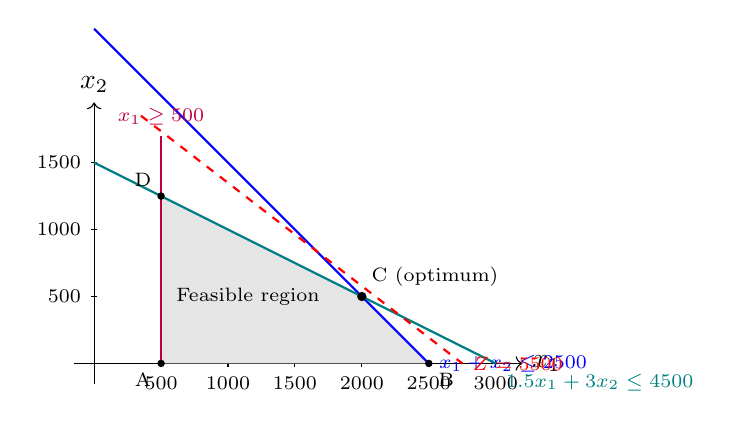
\begin{tikzpicture}[scale=0.85]
  % axes
  \draw[->] (-0.3,0) -- (6.4,0) node[right] {$x_1$};
  \draw[->] (0,-0.3) -- (0,3.9) node[above] {$x_2$};
  \foreach \x/\lbl in {1/500,2/1000,3/1500,4/2000,5/2500,6/3000}
    \draw (\x,0.05) -- (\x,-0.05) node[below,font=\scriptsize] {\lbl};
  \foreach \y/\lbl in {1/500,2/1000,3/1500}
    \draw (0.05,\y) -- (-0.05,\y) node[left,font=\scriptsize] {\lbl};

  % feasible region (scale: 1 unit = 500 t)
  \fill[gray!20] (1,0) -- (5,0) -- (4,1) -- (1,2.5) -- cycle;

  % constraint lines
  \draw[thick,blue] (0,5) -- (5,0) node[right,font=\scriptsize,blue] {$x_1+x_2\leq 2500$};
  \draw[thick,teal] (0,3) -- (6,0) node[below right,font=\scriptsize,teal] {$1.5x_1+3x_2\leq 4500$};
  \draw[thick,purple] (1,0) -- (1,3.4) node[above,font=\scriptsize,purple] {$x_1\geq 500$};

  % iso-profit line through the optimum: 2x1+3x2 = 5500
  \draw[dashed,red,thick] (0.7,3.7) -- (5.5,0) node[right,font=\scriptsize,red] {$Z=5500$};

  % vertices
  \fill (1,0) circle (1.6pt) node[below left,font=\scriptsize] {A};
  \fill (5,0) circle (1.6pt) node[below right,font=\scriptsize] {B};
  \fill (4,1) circle (2pt) node[above right,font=\scriptsize] {C (optimum)};
  \fill (1,2.5) circle (1.6pt) node[above left,font=\scriptsize] {D};

  \node at (2.3,1.0) [font=\scriptsize] {Feasible region};
\end{tikzpicture}
\end{center}

\section{A structured approach to formulating design problems}
\label{sec:structured-formulation}

\subsection{Why structure matters}

The cargo-mix example was formulated directly, with named variables
$x_1$, $x_2$. This works for two variables but breaks down as soon as a
problem involves a set of cargo types, cabin types, or equipment items
whose size is not fixed in advance. A structured formulation — organized
into \emph{sets}, \emph{parameters}, \emph{variables}, and \emph{model} —
scales to any number of items, communicates the model unambiguously to a
reader who was not in the room when it was built, and can be checked for
correctness before a single line of code is written. It also, done well,
gives a near one-to-one correspondence between the mathematical statement
and its implementation, which is the single largest time-saver when
debugging a model that does not solve as expected.

Further, keeping a strict division between the generic model and the data set(s) corresponding to the parameters of the model enables the easy reuse of the same model across many cases and datasets. This is also helpful in model development. You can start with a very simple model just for testing purposes, and then exand this to real cases without touching the model itself.

\subsection{Sets, parameters, variables, and model}

Recast in this structure, the cargo-mix problem reads:

\medskip
\noindent\textbf{Sets}
\begin{align*}
  K  && \text{set of cargo types (cement, brine), indexed by } k
\end{align*}

\noindent\textbf{Parameters}
\begin{align*}
  R_k & && \text{freight rate for cargo type } k \text{ (kEUR/t)} \\
  V_k & && \text{stowage volume per tonne of cargo type } k \text{ (m}^3\text{/t)} \\
  W^{\text{MAX}} & && \text{maximum deadweight (t)} \\
  U^{\text{MAX}} & && \text{maximum hold/tank volume (m}^3\text{)} \\
  Q_k^{\text{MIN}} & && \text{minimum quantity of cargo type } k \text{ (t)}
\end{align*}

\noindent\textbf{Variables}
\begin{align*}
  x_k & && \text{tonnes of cargo type } k \text{ loaded}
\end{align*}

\noindent\textbf{Model}
\begin{align}
  \max \quad & \sum_{k \in K} R_k x_k \notag\\
  \text{s.t.} \quad & \sum_{k \in K} x_k \leq W^{\text{MAX}} \notag\\
  & \sum_{k \in K} V_k x_k \leq U^{\text{MAX}} \notag\\
  & x_C \geq Q_C^{\text{MIN}} \notag\\
  & x_k \geq 0, \quad k \in K \notag
\end{align}

\noindent With $K=\{C,B\}$ this is exactly Equation~\eqref{eq:cargomix};
the value of the structured version only becomes apparent once $|K|$
grows beyond two or three, as it does in Section~\ref{sec:cabin-problem}.

\subsection{Notation conventions}

The choice of symbols is not cosmetic — a consistent scheme makes a model
readable without a legend. The conventions used throughout this
compendium are reflecting the common notation used in the maritime systems design research community, and are summarized below.

\begin{center}
\begin{tabular}{@{}p{0.46\textwidth}p{0.46\textwidth}@{}}
\toprule
Convention & Example \\
\midrule
Uppercase for parameters, lowercase for variables (not without exception) & $R_k$ (parameter), $x_k$ (variable) \\
Prefer single, meaningful letters over acronyms & $C_k^F$ rather than $\mathrm{OPEX}_k$ \\
Letters that recall the underlying quantity & $C$ cost, $P$ price, $V$ speed, $T$ time, $Q$ quantity \\
Subscripts for indices, superscripts for variants of the same quantity & $C_k^I$ investment cost, $C_k^O$ operating cost, for item $k$ \\
$x, y, z$ for variables; $\delta$ for binary variables & $\delta_k \in \{0,1\}$ \\
\bottomrule
\end{tabular}
\end{center}

\section{Application: ship configuration and general arrangement design}
\label{sec:cabin-problem}

\subsection{The cabin arrangement problem}

A recurring class of ship design problem is allocating a scarce resource
— deck area, side length for balconies, tank volume — across a set of
competing uses to maximize revenue. The cabin arrangement problem on a
cruise vessel is a compact instance: choose how many cabins of each type
to build, given a limited total area and a limited length of outer hull
available for balconies.

\medskip
\noindent\textbf{Sets}: 
\begin{align*}
    K & && \text{the set of cabin types, indexed by } k
\end{align*}

\medskip
\noindent\textbf{Parameters}
\begin{align*}
  A_k & && \text{area required per cabin of type } k \text{ (m}^2\text{)} \\
  L_k & && \text{balcony length required per cabin of type } k \text{ (m)} \\
  R_k & && \text{net revenue per cabin of type } k \text{ (kUSD/week)} \\
  A^{\text{TOT}} & && \text{total area available for cabins (m}^2\text{)} \\
  L^{\text{TOT}} & && \text{total outer hull length available for balconies (m)}
\end{align*}

\noindent\textbf{Variables}: $x_k$, the number of cabins of type $k$ built.

\medskip
\noindent\textbf{Model}
\begin{align}
  \max \quad & \sum_{k \in K} R_k x_k \label{eq:cabin-base}\\
  \text{s.t.} \quad & \sum_{k \in K} A_k x_k \leq A^{\text{TOT}} \notag\\
  & \sum_{k \in K} L_k x_k \leq L^{\text{TOT}} \notag\\
  & x_k \geq 0, \quad k \in K \notag
\end{align}

For a concrete instance, take three cabin types: Luxury, First class, and
Standard, with $R = (9,6,4)$ kUSD/week, $A = (20,14,10)$~m$^2$,
$L = (4,3,0)$~m, $A^{\text{TOT}} = 5000$~m$^2$, $L^{\text{TOT}} = 750$~m.
A common additional requirement is that certain cabin types are restricted
to specific decks; here, luxury cabins must be on the two upper decks,
which together offer $A^{\text{UD}} = 3000$~m$^2$. Writing $K^{\text{UD}}
\subseteq K$ for the cabin types restricted to the upper decks, this adds
one further constraint to \eqref{eq:cabin-base}:
\begin{equation}
  \sum_{k \in K^{\text{UD}}} A_k x_k \leq A^{\text{UD}}. \label{eq:cabin-ud}
\end{equation}

\subsection{Solving the model in Python with Xpress}

\subsubsection{Setting up the environment}

The FICO Xpress Python interface (\texttt{xpress}) is used throughout this
course. The free Community license used in the examples caps the problem
size (variables and constraints), which is not a limitation for the
models built in this chapter but will matter for the larger fleet
problems built up over the term project.

\begin{lstlisting}[language=Python]
import xpress as xp
\end{lstlisting}

\subsubsection{From formulation to code}

The point of the structured formulation in Section~\ref{sec:structured-formulation}
is that it maps directly onto the Xpress API: sets become Python
iterables, parameters become dictionaries indexed by the same keys, and
the model statement becomes an objective expression and a list of
constraint expressions built with \texttt{xp.Sum}.

\begin{lstlisting}[language=Python]
K = ["Luxury", "First class", "Standard"]

R = {"Luxury": 9, "First class": 6, "Standard": 4}    # kUSD/week
A = {"Luxury": 20, "First class": 14, "Standard": 10} # m^2
L = {"Luxury": 4,  "First class": 3,  "Standard": 0}  # m

A_TOT = 5000   # m^2
L_TOT = 750    # m
A_UD  = 3000   # m^2, area available on the upper decks
K_UD  = ["Luxury"]

x = {k: xp.var(name=f"x_{k}", lb=0, ub=1000) for k in K}
\end{lstlisting}

\subsubsection{Building and solving the problem}

\begin{lstlisting}[language=Python]
p = xp.problem()
p.addVariable(x)

p.setObjective(xp.Sum(R[k]*x[k] for k in K), sense=xp.maximize)

p.addConstraint(
    xp.Sum(A[k]*x[k] for k in K) <= A_TOT,
    xp.Sum(L[k]*x[k] for k in K) <= L_TOT,
    xp.Sum(A[k]*x[k] for k in K_UD) <= A_UD,
)

p.solve()
\end{lstlisting}

\subsubsection{Retrieving and checking the solution}

\begin{lstlisting}[language=Python]
for k in K:
    print(k, p.getSolution(x[k]))
print("Revenue (kUSD/week):", p.getObjVal())
\end{lstlisting}

The solution is $x^\ast = (150, 50, 130)$ cabins (Luxury, First class,
Standard), with revenue $Z^\ast = 2170$~kUSD/week. All three constraints
are binding: the area constraint uses exactly $20(150)+14(50)+10(130) =
5000$~m$^2$; the balcony constraint uses exactly $4(150)+3(50) =
750$~m; and the upper-deck constraint uses exactly $20(150) =
3000$~m$^2$. This was verified independently with
\texttt{scipy.optimize.linprog} before being written up here.\footnote{The
optimal cabin counts happen to be integers, even though $x_k$ was declared
as a continuous variable. This is a property of this particular numerical
instance, not a general guarantee — see the remark on divisibility in
Section~\ref{sec:lp-assumptions}. In general, a design problem with
genuinely discrete choices requires integer programming, covered later in
the course.}

\subsubsection{Separating data from the model}

As the number of cabin types grows, it becomes worth keeping the
parameters in a spreadsheet or dataframe rather than hard-coded
dictionaries, so that the same model can be re-solved against different
data without touching the formulation:

\begin{lstlisting}[language=Python]
import pandas as pd

df = pd.read_excel("cabindata.xlsx", sheet_name="CabinTypes", index_col="ctID")
K = df.index.tolist()

x = {k: xp.var(name=f"x_{k}", lb=0, ub=1000) for k in K}

p = xp.problem()
p.addVariable(x)
p.setObjective(xp.Sum(df.loc[k, "R"]*x[k] for k in K), sense=xp.maximize)
p.addConstraint(
    xp.Sum(df.loc[k, "A"]*x[k] for k in K) <= A_TOT,
    xp.Sum(df.loc[k, "L"]*x[k] for k in K) <= L_TOT,
)
p.solve()
\end{lstlisting}

This is the pattern to reuse for the fleet capacity problem in assignment
A2, where the number of vessel types and routes is large enough that
hard-coding the data would make the model unreadable.

\subsubsection{A note on Gurobi}

The Gurobi Python interface (\texttt{gurobipy}) follows the same
three-step pattern — declare variables, set an objective, add constraints
— so a model built in Xpress ports with only syntactic changes:

\begin{lstlisting}[language=Python]
import gurobipy as gp
from gurobipy import GRB

m = gp.Model("cabin_arrangement")
x = {k: m.addVar(lb=0, ub=1000, name=f"x_{k}") for k in K}
m.setObjective(gp.quicksum(R[k]*x[k] for k in K), GRB.MAXIMIZE)
m.addConstr(gp.quicksum(A[k]*x[k] for k in K) <= A_TOT)
m.addConstr(gp.quicksum(L[k]*x[k] for k in K) <= L_TOT)
m.addConstr(gp.quicksum(A[k]*x[k] for k in K_UD) <= A_UD)
m.optimize()
\end{lstlisting}

The choice between the two is mostly a licensing question; the modelling
discipline built up in this chapter — sets, parameters, a 1:1 translation
into code, and independent numerical verification of the result — applies
unchanged to either.

\subsection{Discussion: what makes this a general arrangement problem}

The cabin problem is an instance of a more general pattern: a fixed
"footprint" (area, length, volume, weight) is divided among a set of
design elements, each with its own footprint and its own value. The same
structure applies directly to allocating deck area among container bays,
or weather-deck length among cargo cranes. It does \emph{not} apply
directly to problems where the decision is which item goes into which
physical slot — for instance, deciding which of several tank types to
install in each of several physical tank positions on a chemical tanker.
That decision is inherently discrete (a tank either is or is not of a
given type), and formulating it correctly requires binary variables. It
is revisited under integer programming later in the course.

\section{Bridging to solution methods}
\label{sec:bridging}

The graphical method of Section~\ref{sec:cargo-mix} works because a
two-variable problem can be drawn on paper. It does not extend to three
variables, and certainly not to the cabin problem's three cabin types or
to a fleet problem with dozens of vessel types and routes. What does
extend is the underlying geometric idea: the optimum of a linear program
always occurs at a \emph{corner} of the feasible region (formally, a
basic feasible solution), so an optimal algorithm only needs to search
among corners rather than the entire continuum of feasible points.

This is the idea behind the \emph{Simplex method}, developed by
Dantzig in 1947 \citep{dantzig1963}: starting from one corner, move to an
adjacent corner that improves the objective, and repeat until no
adjacent corner improves further. Executing this by hand requires
rewriting the problem in \emph{augmented form} (converting each $\leq$
constraint into an equality by introducing a non-negative \emph{slack
variable}) and organizing the resulting equations into a \emph{tableau}.
The mechanics of the tableau, together with the dual values and
sensitivity ranges that fall out of the optimal tableau almost for free,
are the subject of the next lecture note — worked through on the same
cargo-mix example, and retrieved from the same Xpress \texttt{problem}
object via \texttt{p.getDual()}, \texttt{p.getSlack()}, and
\texttt{p.objsa()}.

\section{Connection to the term project}

Assignment A2 asks each group to formulate a linear program for the
fleet capacity problem introduced in Week 1. The two worked examples in
this chapter are deliberately small enough to solve by hand or check by
inspection; A2 is not. The expectation is the same three-step discipline
demonstrated here: state the problem as sets, parameters, variables, and
model before writing any code; translate that statement into Xpress (or
Gurobi) term for term; and verify the returned solution against the
constraints by hand, on at least one instance, before trusting the model
on the full dataset.


% ch_integer_programming.tex  —  Chapter: Integer programming: binary decisions in fleet renewal and retrofit
% Content only — compiled via main.tex
% Figures in fig/, code in code/
\chapter{Integer programming: binary decisions in fleet renewal and retrofit}
\label{ch:ip-intro}

The previous chapter treated every decision variable as continuous, such as a
cargo quantity, or a number of cabins. These could take any non-negative real
value. \emph{Divisibility} was one of the four defining assumptions of a
linear program, and we saw in the cabin
problem that an integer-valued optimum can appear in a continuous LP
purely by coincidence (and thus, no integer-specific constraints are needed). 
However, we cannot generally assume this for any arbitrary discrete design problem. 
In particular for yes/no problems, such as whether to install a particular retrofit package on a
particular vessel, whether to build a salmon farm at one location or two, whether
a given tank position holds one product type or another. Modelling them as continuous variables that happen to
settle at $0$ or $1$ is not a strategy that can be relied on.

This chapter introduces \emph{integer programming}, and its most common
special case, \emph{binary integer programming}, as the natural extension
of the LP problem, with a focus on discrete decisions.
Section~\ref{sec:binary-modelling} develops a small toolbox of binary
modelling constructs --- mutually exclusive choices, conditional
decisions, and installation--use linkages --- that recur throughout ship
design optimization. Section~\ref{sec:knapsack} applies this toolbox to
the classical knapsack problem, introducing the central practical concern
of this chapter: a correct formulation is not automatically a good one,
and some formulations solve far more easily than others.
Section~\ref{sec:bnb} develops branch-and-bound, the exact solution method
underlying every commercial and open-source MILP solver, including
Xpress. Section~\ref{sec:fleet-retrofit} brings all of this together in a
single, sizeable worked example: choosing which emission-abatement
retrofits to install, on which vessel, and when, to meet a
stepwise-tightening fleet emissions cap at minimum cost --- the fleet
renewal and retrofit problem that anchors assignment A4.

\section{From continuous to discrete decisions}
\label{sec:ip-intro-sec}

\subsection{Where the linear program breaks down}

A number of cabins, an on/off retrofit decision, or a choice between two
candidate factory sites is not a divisible quantity: $x=0.4$ of a
heat-recovery unit installed is not a meaningful design. When a decision
variable is restricted to take only integer values --- or, in the common
special case of a yes/no decision, only the values $0$ and $1$ --- the
resulting problem is an \emph{integer program}. Everything else about the
model is unchanged: objective and constraints remain linear in the
decision variables, so the structured formulation discipline developed for
linear programs (sets, parameters, variables, model) applies without
modification. Only the domain of the variables changes.

\subsection{Pure, mixed, and binary integer programs}
\label{sec:ip-types}

It is useful to distinguish three variants, since the terminology recurs
throughout the literature and in solver documentation.

\begin{description}
  \item[(Pure) integer programming, IP.] All decision variables are
  restricted to integers, $x_j \in \mathbb{Z}_{\geq 0}$.
  \item[Mixed integer programming, MIP.] Some variables are restricted to
  integers, others remain continuous. Most realistic ship design models
  are of this type: a design decision might be integer (number of tanks)
  while an associated operating quantity remains continuous (tonnes of
  product carried in each tank).
  \item[Binary integer programming, BIP.] Every integer variable is
  further restricted to $\{0,1\}$. This is overwhelmingly the most common
  case in design and configuration problems, because most genuinely
  discrete design decisions are yes/no choices at the level the model
  represents them.
\end{description}

A general mixed-integer linear program can be written
\begin{align}
  \max \quad & Z = \sum_{j=1}^{n} c_j x_j \notag\\
  \text{s.t.} \quad & \sum_{j=1}^{n} a_{ij}x_j \leq b_i, \quad i=1,\ldots,m \notag\\
  & x_j \geq 0, \quad j=1,\ldots,n \notag\\
  & x_j \in \mathbb{Z}, \quad j \in J \subseteq \{1,\ldots,n\}, \notag
\end{align}
where $J$ is the subset of variables restricted to integers ($J=\{1,\ldots,n\}$
for a pure IP, and $x_j \in \{0,1\}$ for $j\in J$ for a BIP).

\subsection{The LP relaxation}
\label{sec:lp-relaxation}

Dropping the integrality restriction on every $x_j\in J$ and solving the
resulting ordinary linear program is called the \emph{LP relaxation} of
the integer program. Because the LP relaxation is solved over a
\emph{larger} feasible region than the original problem (every
integer-feasible point is also LP-feasible, but not vice versa), its
optimal value is always at least as good as the integer program's --- an
upper bound for a maximization problem, a lower bound for a minimization
problem. This bounding property is the single most important tool in
solving integer programs, and underlies the branch-and-bound method of
Section~\ref{sec:bnb}.

It also explains an apparent paradox: an integer program is, for equal
numbers of variables and constraints, almost always \emph{harder} to
solve than its LP relaxation, even though it has \emph{fewer} feasible
points. Removing points from a feasible region does nothing to make a
linear program's own structure --- convexity, the guarantee that an
optimum sits at a vertex --- any easier to exploit; it only removes the
guarantee that the Simplex method's vertex-to-vertex search will land on
a feasible point at all. Solving an integer program therefore generally
means solving \emph{many} LP relaxations, not one. (There are well-known
exceptions: the transportation problem introduced later in the course
happens to have an LP relaxation whose optimal basic solutions are
automatically integer, for any integer supply and demand data --- a
property of that particular constraint structure, not something to expect
in general.)

\section{Modelling logical relationships with binary variables}
\label{sec:binary-modelling}

A binary variable $\delta_k\in\{0,1\}$ is most useful not as a quantity
but as an \emph{indicator}: $\delta_k=1$ if some discrete choice $k$ is
made, $\delta_k=0$ otherwise. A small number of linear constraint patterns,
combined, can express most of the logical relationships that arise
between such choices. Table~\ref{tab:binary-constructs} collects the
constructs used repeatedly in this chapter and in the term project; in
each case $x_A,x_B\in\{0,1\}$ are indicators for decisions $A$ and $B$.

\begin{table}[htbp]
  \centering
  \caption{Standard binary modelling constructs.}
  \label{tab:binary-constructs}
  \begin{tabular}{@{}p{0.27\textwidth}p{0.22\textwidth}p{0.4\textwidth}@{}}
    \toprule
    Relationship & Constraint & Ship design example \\
    \midrule
    At most one of $A,B$ (mutually exclusive) & $x_A+x_B\leq 1$ & Build the salmon fodder factory at Fr{\o}ya \emph{or} Bjugn, not both \\
    At most $k$ of $n$ options & $\sum_{k} x_k \leq k^{\max}$ & Install at most two of the four available retrofits \\
    Exactly one of $n$ options (partition) & $\sum_{k} x_k = 1$ & Choose exactly one propulsion configuration \\
    $A$ implies $B$ (``if $A$ then $B$'') & $x_A - x_B \leq 0$ & If a propeller is fitted, a shaft must be too \\
    $B$ only if $A$ (converse implication) & $x_B - x_A \leq 0$ & An abatement option is only in use if it has been installed \\
    $A$ and $B$ logically equivalent & $x_A = x_B$ & Installation and use coincide exactly \\
    \bottomrule
  \end{tabular}
\end{table}

The last two rows are easy to confuse: ``$A$ implies $B$'' and ``$B$ only
if $A$'' are converse statements, and the correct constraint direction
depends on which one is meant. A useful check is to ask which combination
is being ruled out: $x_A-x_B\leq0$ rules out $x_A=1,x_B=0$ (installing $A$
without $B$); $x_B-x_A\leq0$ rules out $x_B=1,x_A=0$ (using $B$ without
$A$ ever having been installed). Section~\ref{sec:fleet-retrofit} uses
exactly this second pattern to tie the use of an abatement option to its
installation.

A related and very common construct links a binary decision to a
continuous or bounded quantity: ``if $\delta=0$ then $y=0$'' is enforced
by $y\leq M\delta$ for a suitably large constant $M$ (a \emph{big-M}
constraint). This is often unavoidable, but it comes at a cost: the LP
relaxation of $y\leq M\delta$ allows $y$ to be as large as $M\delta$ for
any fractional $\delta$, which can be costly for the
branch-and-bound algorithm. Thus choosing the smallest possible
$M$ --- or, where possible, avoiding the construct altogether in favour of
an exact algebraic relationship --- is often a better solution.
Section~\ref{sec:fleet-retrofit} describes a case where a
big-M constraint used in an existing model turns out to be unnecessary,
and removing it tightens the LP relaxation substantially.

\section{The 0/1 knapsack problem}
\label{sec:knapsack}

\subsection{Formulation}

The \emph{0/1 knapsack problem} is the simplest genuine binary integer
program, and a useful reference point before tackling larger models:
choose a subset of $n$ available items, each with a value $R_k$ and a
resource requirement $W_k$, to maximize total value without exceeding a
fixed resource budget $W^{\max}$.

A simple and easy-to-understand illustration of this problem is yourself packing your suitcase for vacation. The suitcase has a given volume and a (airline defined) maximum weight. Thus, making your choices strikes a balance between the weight and volume of each item vs. the value this item will have for you for the next week. The bikini and the shorts are easy, both small, light and valuable (given that your are not traveling to Tr{\o}ndelag), while your SUP board may be more on the balance.

\medskip
\noindent\textbf{Sets}: $K$, the set of candidate items, indexed by $k$.

\medskip
\noindent\textbf{Parameters}
\begin{align*}
  R_k & &&\text{value of item } k \\
  W_k & &&\text{resource requirement of item } k \\
  W^{\max} & &&\text{available resource budget}
\end{align*}

\noindent\textbf{Variables}: $x_k\in\{0,1\}$, $1$ if item $k$ is selected.

\medskip
\noindent\textbf{Model}
\begin{align}
  \max \quad & \sum_{k\in K} R_k x_k \label{eq:knapsack}\\
  \text{s.t.} \quad & \sum_{k\in K} W_k x_k \leq W^{\max} \notag\\
  & x_k \in \{0,1\}, \quad k\in K. \notag
\end{align}

Every constraint here has exactly the same anatomy as the deadweight and
volume constraints of the earlier cargo-mix problem; only the domain of
$x_k$ has changed.

\subsection{A retrofit-selection example, and why greedy fails}

Consider a shipowner choosing which of three available energy-saving
retrofits to install on a single vessel within a fixed CAPEX budget of
10~mNOK: a waste-heat recovery system (WHR), a new hull coating (HC), and
a propeller upgrade (PU). Table~\ref{tab:knapsack-retrofit} gives the
estimated NPV of each measure and its CAPEX.

\begin{table}[htbp]
\centering
\caption{Candidate retrofit measures for the knapsack example.}
\label{tab:knapsack-retrofit}
\begin{tabular}{@{}lccc@{}}
\toprule
Measure & NPV (mNOK) & CAPEX (mNOK) & NPV/capex \\
\midrule
Waste-heat recovery (WHR) & 10 & 6 & 1.67 \\
Hull coating (HC) & 6 & 5 & 1.20 \\
Propeller upgrade (PU) & 6 & 5 & 1.20 \\
\bottomrule
\end{tabular}
\end{table}

A natural heuristic is to rank items by value per unit of resource
consumed and install them greedily until the budget runs out: WHR has the
best ratio (1.67) and fits within the 10~mNOK budget on its own, leaving
4~mNOK --- not enough for HC or PU (5~mNOK each). The greedy heuristic
therefore installs WHR alone, for a total NPV of 10~mNOK.

This is not the optimal integer solution. Installing HC and PU together
costs exactly 10~mNOK and delivers an NPV of $6+6=12$~mNOK, twenty percent
higher, confirmed by exhaustive enumeration of all $2^3=8$ subsets. The
reason greedy fails here is that it is exactly optimal for the
\emph{continuous relaxation} of the knapsack problem (the ``fractional
knapsack''): sorting by ratio and filling the budget, taking a fraction of
the last item if necessary, does solve the LP relaxation of
\eqref{eq:knapsack} optimally. Doing so here gives a fractional relaxation
value of 14.8~mNOK (all of WHR, plus 80\% of HC) --- confirming that the
LP relaxation is a valid upper bound on the true integer optimum of 12, as
Section~\ref{sec:lp-relaxation} predicts, and illustrating why the greedy
allocation, forced to be integral only because it cannot use a fraction of
a physical retrofit, leaves value on the table: it commits early to the
best-ratio item and never reconsiders that choice once a poor fit is
discovered.

\subsection{Solving the exact problem}

\begin{lstlisting}[language=Python]
import xpress as xp

K = ["WHR", "HC", "PU"]
R = {"WHR": 10, "HC": 6, "PU": 6}      # NPV, mNOK
W = {"WHR": 6,  "HC": 5, "PU": 5}      # capex, mNOK
W_MAX = 10

x = {k: xp.var(vartype=xp.binary, name=f"x_{k}") for k in K}

p = xp.problem()
p.addVariable(x)
p.setObjective(xp.Sum(R[k]*x[k] for k in K), sense=xp.maximize)
p.addConstraint(xp.Sum(W[k]*x[k] for k in K) <= W_MAX)
p.solve()

for k in K:
    print(k, p.getSolution(x[k]))
print("NPV (mNOK):", p.getObjVal())
\end{lstlisting}

The optimal solution installs HC and PU, for an NPV of 12~mNOK, exactly
the exhaustive-enumeration result above (verified independently with a
brute-force search over all $2^3$ subsets before being written up here).
Two modelling details are worth noting for later use: the variable is
declared directly with \texttt{vartype=xp.binary} rather than as a
continuous variable with $[0,1]$ bounds, which is both clearer and lets
the solver apply integer-specific presolve reductions immediately; and,
unlike the LP examples of the previous chapter, there is no guarantee
here that a continuous relaxation happens to be integral --- as just
shown, it is not.

The general 0/1 knapsack problem is NP-hard: no algorithm is known that
solves every instance in time polynomial in $n$, and none is expected to
exist. In practice this rarely matters --- an efficient pseudo-polynomial
dynamic programming algorithm (indexing subproblems by budget consumed)
solves knapsack instances of practical size quickly, and Xpress solves
problems very much larger than this chapter's examples in a fraction of a
second, using the branch-and-bound method developed next. The knapsack
problem's role here is pedagogical: it is the smallest instance in which
the \emph{integrality gap} --- the difference between the LP relaxation
bound and the true integer optimum --- is visible and easy to compute by
hand, and every larger model in this chapter and the term project
contains a knapsack-like resource constraint at its core, extended with
the logical constructs of Section~\ref{sec:binary-modelling}. The fleet
retrofit problem of Section~\ref{sec:fleet-retrofit}, in particular, is a
knapsack decision --- which abatement options to install, under a cost
budget --- repeated over every vessel and time period, and coupled across
both by a shared emissions constraint.

\section{Branch and bound: an exact solution method}
\label{sec:bnb}

\subsection{Three insights and three steps}

Branch-and-bound solves an integer program by implicitly enumerating its
feasible solutions, without ever listing them explicitly. The method
rests on three observations, each a direct consequence of the LP
relaxation property of Section~\ref{sec:lp-relaxation}.

\begin{enumerate}
  \item Adding a constraint to a problem can only leave its optimal value
  unchanged or make it worse; it can never improve it, because the
  feasible region can only shrink.
  \item An infeasible problem remains infeasible under any additional
  constraint --- there is nothing left to shrink.
  \item Restricting a continuous variable to an integer value is itself
  an added constraint, from the point of view of the LP relaxation that
  ignores it.
\end{enumerate}

Together these three facts mean that if a sub-problem's LP relaxation is
already worse than the best integer solution found so far (the
\emph{incumbent}), no amount of further restriction --- including forcing
more variables to be integer --- can recover it. This is the basis for
discarding, or \emph{fathoming}, entire branches of the search tree
without exploring them.

The method proceeds in three repeated steps.

\begin{enumerate}
  \item[\textbf{Branch.}] Pick a variable $x_j$, $j\in J$, whose value in
  the current LP relaxation is fractional, and create two sub-problems by
  adding $x_j\leq\lfloor x_j^\ast\rfloor$ to one and
  $x_j\geq\lceil x_j^\ast\rceil$ to the other (for a binary variable, this
  is simply $x_j=0$ and $x_j=1$).
  \item[\textbf{Bound.}] Solve the LP relaxation of each sub-problem. Its
  optimal value bounds the best integer solution attainable in that
  branch.
  \item[\textbf{Fathom.}] Discard a branch, without exploring it further,
  if any of the following holds: (a) its LP bound is no better than the
  current incumbent; (b) its LP relaxation is infeasible; (c) its LP
  relaxation is already integer-feasible --- in which case it is itself a
  candidate solution, and becomes the new incumbent if it improves on the
  current one.
\end{enumerate}

The search terminates when every branch has been fathomed; the incumbent
at that point is the proven optimal solution
\citep{landdoig1960}. Xpress, like every commercial MILP solver,
implements a highly refined version of this idea internally, adding
automatic cutting planes and heuristics not covered here; the manual
example below is for building intuition, not for how these problems are
solved in practice --- in practice, \texttt{p.solve()} is enough.

\subsection{Worked example: locating a farm and a factory}
\label{sec:bnb-example}

Marlax is considering new salmon farms at Fr{\o}ya, at Bjugn, or both, and
a single processing factory that can only be built alongside one of the
two farms. The investment budget is 10~mEUR; Table~\ref{tab:aqua-data}
gives the net present value and required capital for each of the four
binary decisions.

\begin{table}[htbp]
\centering
\caption{Investment decisions for the aquaculture location problem.}
\label{tab:aqua-data}
\begin{tabular}{@{}clcc@{}}
\toprule
Variable & Decision & NPV (mEUR) & Capex (mEUR) \\
\midrule
$x_1$ & Build farm at Fr{\o}ya & 9 & 6 \\
$x_2$ & Build farm at Bjugn & 5 & 3 \\
$x_3$ & Build factory at Fr{\o}ya & 6 & 5 \\
$x_4$ & Build factory at Bjugn & 4 & 2 \\
\bottomrule
\end{tabular}
\end{table}

\begin{align}
  \max \quad & 9x_1+5x_2+6x_3+4x_4 \label{eq:aqua}\\
  \text{s.t.} \quad & 6x_1+3x_2+5x_3+2x_4 \leq 10 && \text{(capex budget)} \notag\\
  & x_3+x_4 \leq 1 && \text{(at most one factory)} \notag\\
  & x_3 \leq x_1 && \text{(factory at Fr\o ya only if a farm is built there)} \notag\\
  & x_4 \leq x_2 && \text{(factory at Bjugn only if a farm is built there)} \notag\\
  & x_j \in \{0,1\}, \quad j=1,\ldots,4. \notag
\end{align}

The last two constraints are exactly the ``$B$ only if $A$'' construct of
Table~\ref{tab:binary-constructs}, written here as $x_3-x_1\leq0$ and
$x_4-x_2\leq0$; the second constraint is the mutually-exclusive construct
restricted to the two factory variables.

Figure~\ref{fig:bnb-tree} shows the full search tree, with every LP
relaxation solved and verified with \texttt{scipy.optimize.linprog}. The
root relaxation gives $Z=16.5$ at $x=(0.83,1,0,1)$: only $x_1$ is
fractional, so the tree branches on $x_1$ first, exploring the branch
nearer the fractional value ($x_1=1$) before the other. Each subsequent
branch is chosen the same way, on the (in this example, always unique)
fractional variable in the parent's solution.

Branch $x_1=0$ happens to be integer-feasible immediately
($x=(0,1,0,1)$, $Z=9$), but the $x_1=1$ side of the tree is explored to
completion first, producing a better integer solution before this
branch's fathoming even becomes relevant. Branching on $x_2$, then $x_4$,
then $x_3$ within the $x_1=1$ subtree eventually reaches $x=(1,1,0,0)$,
$Z=14$, integer and feasible: the new incumbent. Its sibling ($x_3=1$) is
infeasible (the budget constraint alone forces $x_4<0$), and one level up,
the $x_2=0$ branch's own bound of 13.8 is now below the incumbent of 14
and is fathomed without any further branching. Finally, the earlier
$x_1=0$ solution, at $Z=9$, is fathomed for the same reason. Every branch
is now closed, so $x^\ast=(1,1,0,0)$, $Z^\ast=14$ is the proven optimum:
build farms at both Fr{\o}ya and Bjugn, and no factory at either. This was
cross-checked by exhaustive enumeration of all 16 combinations.

Figure~\ref{fig:bnb-tree} shows the full search tree, with every LP
relaxation solved and verified with \texttt{scipy.optimize.linprog}, in
the order a manual search would naturally follow: explore the lower branch
of each split ($x_j=0$) before the upper one ($x_j=1$). The root
relaxation gives $Z=16.5$ at $x=(0.83,1,0,1)$: only $x_1$ is fractional,
so the tree branches on $x_1$.

$x_1=0$ is evaluated first ($N_1$: $x=(0,1,0,1)$, $Z=9$) and is already
integer-feasible, so it is fathomed immediately and --- being the first
integer-feasible solution found --- becomes the incumbent. The search
then moves to $x_1=1$ ($N_2$: $Z=16.2$, $x=(1,0.8,0,0.8)$), whose bound
still exceeds the incumbent of 9, so it is branched further, on $x_2$.
Its $x_2=0$ child ($N_3$: $Z=13.8$) also still exceeds 9 and must itself
be branched, on $x_3$: one child is integer ($N_5$: $x=(1,0,0,0)$,
$Z=9$), which ties but does not beat the incumbent and so does not
replace it; the other ($N_6$, $x_3=1$) is infeasible. Back at $N_2$'s
other child, $x_2=1$ ($N_4$: $Z=16.0$), branching on $x_4$ then $x_3$
eventually reaches $N_9$: $x=(1,1,0,0)$, $Z=14$, integer --- and, since
$14>9$, this replaces the incumbent. $N_9$'s sibling ($N_{10}$, $x_3=1$)
is infeasible, and $N_7$'s other child ($N_8$, $x_4=1$) is infeasible
too. Every branch is now closed, so $x^\ast=(1,1,0,0)$, $Z^\ast=14$ is
the proven optimum: build farms at both Fr{\o}ya and Bjugn, and no
factory at either. This was cross-checked by exhaustive enumeration of
all 16 combinations.

A different exploration order changes how much of the tree needs
visiting, but never the answer. Branching toward the nearer integer each
time --- here, $x_1=1$ before $x_1=0$, since $0.83$ rounds to $1$ ---
would reach $N_9$ and its $Z=14$ almost immediately, and would then close
$N_3$ by bound alone ($13.8<14$) without ever needing to open $N_5$ or
$N_6$: the same proven optimum, at the cost of two fewer nodes explored.
Neither order is ``more correct''; branch-and-bound guarantees the same
answer regardless, and different solvers, and different students working
by hand, may well take different paths to it.

\begin{figure}[htbp]
\centering
\resizebox{\textwidth}{!}{%
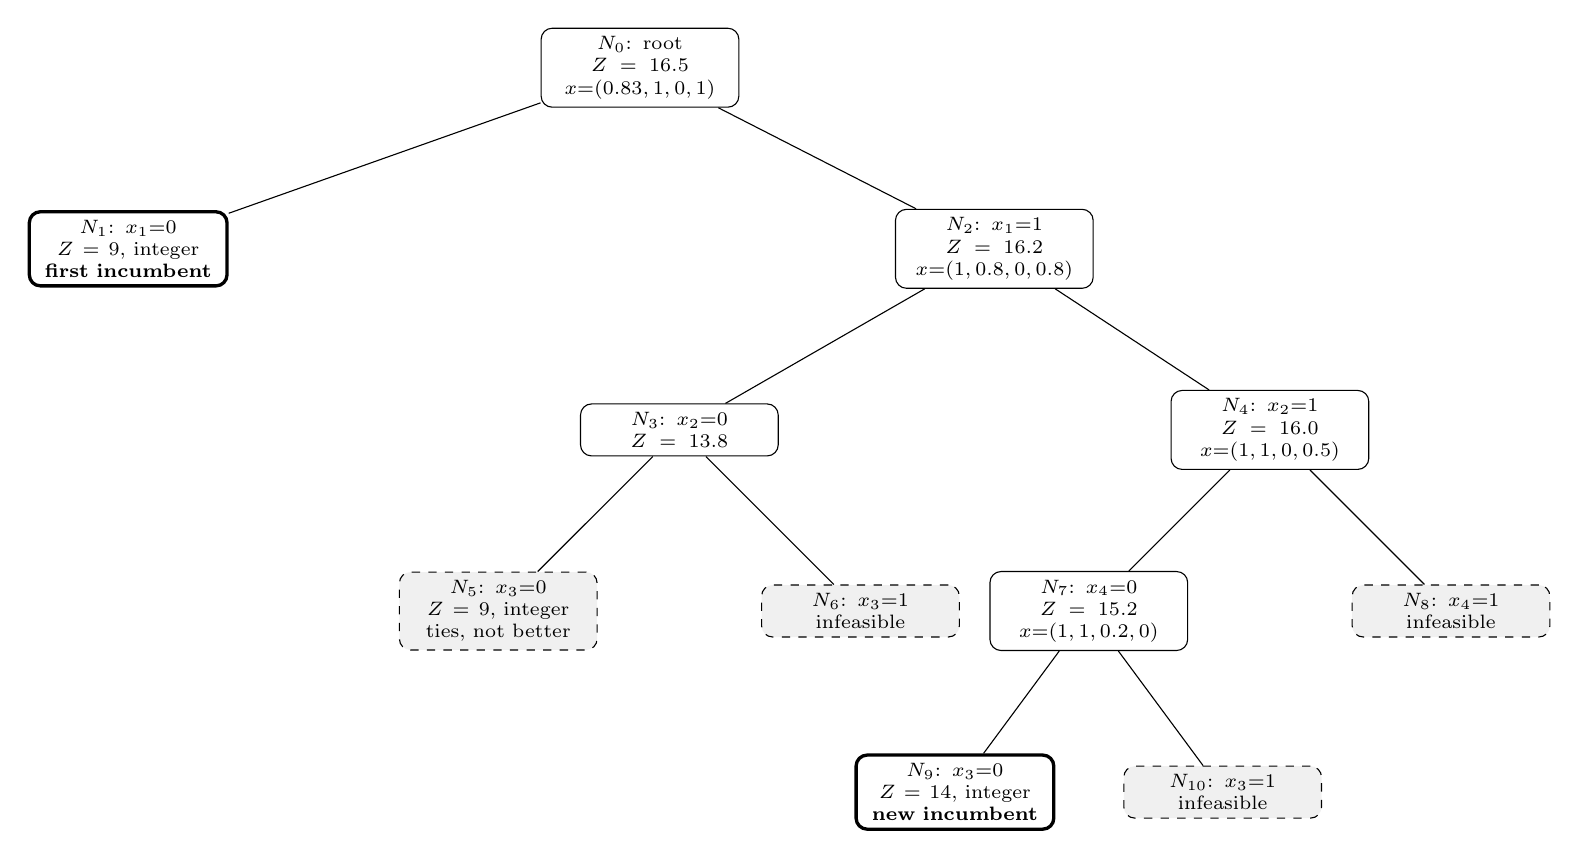
\begin{tikzpicture}[
  every node/.style={font=\scriptsize, text width=2.3cm, align=center},
  box/.style={draw, rectangle, rounded corners, inner sep=3pt},
  fathom/.style={box, dashed, fill=gray!12},
  incumbent/.style={box, very thick}
]
\node[box] (N0) at (0,0) {$N_0$: root\\$Z=16.5$\\$x{=}(0.83,1,0,1)$};

\node[incumbent] (N1) at (-6.5,-2.3) {$N_1$: $x_1{=}0$\\$Z=9$, integer\\\textbf{first incumbent}};
\node[box] (N2) at (4.5,-2.3) {$N_2$: $x_1{=}1$\\$Z=16.2$\\$x{=}(1,0.8,0,0.8)$};

\node[box] (N3) at (0.5,-4.6) {$N_3$: $x_2{=}0$\\$Z=13.8$};
\node[box] (N4) at (8,-4.6) {$N_4$: $x_2{=}1$\\$Z=16.0$\\$x{=}(1,1,0,0.5)$};

\node[fathom] (N5) at (-1.8,-6.9) {$N_5$: $x_3{=}0$\\$Z=9$, integer\\ties, not better};
\node[fathom] (N6) at (2.8,-6.9) {$N_6$: $x_3{=}1$\\infeasible};

\node[box] (N7) at (5.7,-6.9) {$N_7$: $x_4{=}0$\\$Z=15.2$\\$x{=}(1,1,0.2,0)$};
\node[fathom] (N8) at (10.3,-6.9) {$N_8$: $x_4{=}1$\\infeasible};

\node[incumbent] (N9) at (4.0,-9.2) {$N_9$: $x_3{=}0$\\$Z=14$, integer\\\textbf{new incumbent}};
\node[fathom] (N10) at (7.4,-9.2) {$N_{10}$: $x_3{=}1$\\infeasible};

\draw (N0) -- (N1);
\draw (N0) -- (N2);
\draw (N2) -- (N3);
\draw (N2) -- (N4);
\draw (N3) -- (N5);
\draw (N3) -- (N6);
\draw (N4) -- (N7);
\draw (N4) -- (N8);
\draw (N7) -- (N9);
\draw (N7) -- (N10);
\end{tikzpicture}%
}
\caption{Branch-and-bound tree for the aquaculture location problem, explored in the order $x_j=0$ before $x_j=1$ at each split. Dashed nodes are fathomed without becoming (or replacing) the incumbent; bold nodes mark the incumbent at the point it is set.}
\label{fig:bnb-tree}
\end{figure}

The result is a useful reminder that a positive individual NPV --- both
factory options have one --- does not guarantee inclusion in the optimal
solution once a shared budget constraint is taken into consideration. Both factories
compete for the same 10 mEUR, and the second farm
wins.

\section{Application: fleet renewal and retrofit under a tightening emissions cap}
\label{sec:fleet-retrofit}

\subsection{Problem context}

Before we go onto specific regulatory schemes, we will first just consider a generic set of requirements that implies that a fleet's total emissions must decline against a schedule that tightens overall emissions year on year. A shipowner facing such a
schedule can respond, per vessel, by retrofitting an emission-abatement
technology or by replacing the vessel outright with a lower-emission
newbuild. The latter can, for simplicity, be modelled as a retrofit with a 100\%
reduction and a correspondingly larger investment cost, so a single
formulation covers both (assuming replacemnt with a similar vessel). The owner must decide what
abatement technology to install on which ship, and in what time period, balancing an installation cost against an annual operating
cost and an emissions benefits to comply with the fleet-wide cap that becomes
stricter every year.

\subsection{A first formulation}
\label{sec:fleet-model-v1}

\medskip
\noindent\textbf{Sets}
\begin{align*}
  V & &&\text{vessels in the fleet, indexed by } v \\
  A & &&\text{available emission-abatement options, indexed by } a \\
  T & &&\text{time periods in the planning horizon, indexed by } t
\end{align*}

\noindent\textbf{Parameters}
\begin{align*}
  E_v & &&\text{emissions of vessel } v \text{ with no abatement installed} \\
  \gamma_a & &&\text{emission-reduction fraction achieved by option } a \\
  C_a^I & &&\text{installation cost of option } a \\
  C_a^O & &&\text{annual operating cost of option } a, \text{once installed} \\
  E_t^{\text{TOT}} & &&\text{fleet-wide allowed emissions in period } t
\end{align*}

\noindent\textbf{Variables}
\begin{align*}
  x_{vat}\in\{0,1\} & &&1 \text{ if option } a \text{ is installed on vessel } v \text{ in period } t \\
  y_{vat}\in\{0,1\} & &&1 \text{ if option } a \text{ is in use on vessel } v \text{ in period } t
\end{align*}

\noindent\textbf{Model}
\begin{align}
  \min \quad & \sum_{v\in V}\sum_{a\in A}\sum_{t\in T} \left(C_a^I x_{vat} + C_a^O y_{vat}\right) \label{eq:fleet-obj}\\
  \text{s.t.} \quad
  & \sum_{v\in V}\left(E_v - \sum_{a\in A}\gamma_a E_v y_{vat}\right) \leq E_t^{\text{TOT}}, && t \in T \label{eq:fleet-c1}\\
  & \sum_{t\in T} x_{vat} \leq 1, && v\in V, a\in A \label{eq:fleet-c2}\\
  & M\sum_{t\in T}x_{vat} \geq \sum_{t\in T}y_{vat}, && v\in V, a\in A \label{eq:fleet-c3}\\
  & y_{vat} \geq x_{vat}, && v\in V, a\in A, t\in T \label{eq:fleet-c4}\\
  & y_{vat} \geq y_{va,t-1}, && v\in V, a\in A, t\in T\setminus\{0\} \label{eq:fleet-c5}\\
  & y_{vat} - y_{va,t-1} = x_{vat}, && v\in V, a\in A, t\in T\setminus\{0\} \label{eq:fleet-c6}\\
  & x_{va,N-1} = 0, && v\in V, a\in A \label{eq:fleet-c7}\\
  & x_{vat}, y_{vat} \in \{0,1\}, && v\in V, a\in A, t\in T. \notag
\end{align}

Constraint \eqref{eq:fleet-c1} is the emissions cap. \eqref{eq:fleet-c2}
allows each option to be installed on each vessel at most once.
\eqref{eq:fleet-c3} is a big-M linking constraint, using the constructs of
Section~\ref{sec:binary-modelling}: because \eqref{eq:fleet-c2} already
forces $\sum_t x_{vat}\in\{0,1\}$, this says that $y_{vat}$ can only be
positive in \emph{some} period if $a$ is installed on $v$ in \emph{some}
period. \eqref{eq:fleet-c4} forces use to start no later than
installation. \eqref{eq:fleet-c5} forces use, once started, to persist.
\eqref{eq:fleet-c6} ties the two together in every period after the
first: use switches on ($y_{vat}=1$ while $y_{va,t-1}=0$) exactly when
installation happens ($x_{vat}=1$). \eqref{eq:fleet-c7} disallows
installing anything in the final period, since there would be no
operating periods left to recover the cost.

\subsection{A worked instance}
\label{sec:fleet-worked}

\begin{lstlisting}[language=Python]
import xpress as xp
import pandas as pd

def fleet_retrofit_model(dfV, dfA, dfT, bigM=1000):
    V, A, T = dfV.index, dfA.index, dfT.index

    x = {(v,a,t): xp.var(vartype=xp.binary, name=f"x_{v}_{a}_{t}")
         for v in V for a in A for t in T}
    y = {(v,a,t): xp.var(vartype=xp.binary, name=f"y_{v}_{a}_{t}")
         for v in V for a in A for t in T}

    p = xp.problem()
    p.addVariable(x, y)

    totCost = xp.Sum(dfA.C_I[a]*x[v,a,t] + dfA.C_O[a]*y[v,a,t]
                      for v in V for a in A for t in T)
    p.setObjective(totCost, sense=xp.minimize)

    # Emissions cap
    c1 = [xp.Sum(dfV.E[v] - xp.Sum(dfA.gamma[a]*dfV.E[v]*y[v,a,t] for a in A)
                 for v in V) <= dfT.E_req[t]
          for t in T]

    # Install at most once
    c2 = [xp.Sum(x[v,a,t] for t in T) <= 1 for a in A for v in V]

    # Big-M link: some use only if installed at some point
    c3 = [bigM*xp.Sum(x[v,a,t] for t in T) >= xp.Sum(y[v,a,t] for t in T)
          for a in A for v in V]

    # Use starts no later than installation
    c4 = [y[v,a,t] >= x[v,a,t] for t in T for a in A for v in V]

    # Use, once started, persists
    c5 = [y[v,a,t] >= y[v,a,t-1] for t in T[1:] for a in A for v in V]

    # Use switches on exactly when installation happens
    c6 = [y[v,a,t] - y[v,a,t-1] == x[v,a,t]
          for t in T[1:] for a in A for v in V]

    # No installation in the final period
    c7 = [x[v,a,T[-1]] == 0 for a in A for v in V]

    p.addConstraint(c1, c2, c3, c4, c5, c6, c7)
    p.solve()
    return p, x, y
\end{lstlisting}

This is a direct, one-for-one implementation of the model in
Section~\ref{sec:fleet-model-v1}. Three identical
vessels ($E_v=100$ for $v=1,2,3$) face the eight-period emissions cap in
Table~\ref{tab:fleet-cap}, tightening from 290 in period 0 (against an
unabated fleet total of 300) to 40 in the final period, and choose among
the three abatement options in Table~\ref{tab:fleet-options}.

\begin{table}[htbp]
\centering
\caption{Abatement option data for the worked fleet instance.}
\label{tab:fleet-options}
\begin{tabular}{@{}lccc@{}}
\toprule
Option & $\gamma_a$ & $C_a^I$ & $C_a^O$ \\
\midrule
$a_1$ & 0.3 & 20 & 3 \\
$a_2$ & 0.5 & 40 & 4 \\
$a_3$ & 1.0 & 110 & 5 \\
\bottomrule
\end{tabular}
\end{table}

\begin{table}[htbp]
\centering
\caption{Fleet-wide emissions cap by period.}
\label{tab:fleet-cap}
\begin{tabular}{@{}ccccccccc@{}}
\toprule
$t$ & 0 & 1 & 2 & 3 & 4 & 5 & 6 & 7 \\
\midrule
$E_t^{\text{TOT}}$ & 290 & 280 & 260 & 200 & 150 & 120 & 80 & 40 \\
\bottomrule
\end{tabular}
\end{table}

\begin{lstlisting}[language=Python]
dfV = pd.DataFrame({'E': [100, 100, 100]}, index=['v1','v2','v3'])
dfA = pd.DataFrame({'gamma': [0.3, 0.5, 1.0],
                     'C_I':   [20, 40, 110],
                     'C_O':   [3, 4, 5]}, index=['a1','a2','a3'])
dfT = pd.DataFrame({'E_req': [290,280,260,200,150,120,80,40]})

p, x, y = fleet_retrofit_model(dfV, dfA, dfT)
print("Total cost:", p.getObjVal())
\end{lstlisting}

Table~\ref{tab:fleet-result} gives the resulting schedule, solved to
proven optimality and cross-checked with an independent MILP solve
outside Xpress before being written up here.

\begin{table}[htbp]
\centering
\caption{Optimal installation and cost schedule for the worked instance (total cost 309).}
\label{tab:fleet-result}
\begin{tabular}{@{}cp{0.28\textwidth}rrrrr@{}}
\toprule
$t$ & Installed & $C_a^I$ & $C_a^O$ & Emissions & $E_t^{\text{TOT}}$ & Period cost \\
\midrule
0 & $a_3$ on $v_1$ & 110 & 5 & 200 & 290 & 115 \\
1 & --- & 0 & 5 & 200 & 280 & 5 \\
2 & --- & 0 & 5 & 200 & 260 & 5 \\
3 & --- & 0 & 5 & 200 & 200 & 5 \\
4 & $a_2$ on $v_2$ & 40 & 9 & 150 & 150 & 49 \\
5 & $a_1$ on $v_2$ & 20 & 12 & 120 & 120 & 32 \\
6 & $a_1,a_2$ on $v_3$ & 60 & 19 & 40 & 80 & 79 \\
7 & --- & 0 & 19 & 40 & 40 & 19 \\
\bottomrule
\end{tabular}
\end{table}

Total cost over the horizon is 309, reached by fully decarbonizing one
vessel early (period 0, since the cap tightens fastest relative to
installed capability there) and layering cheaper, partial-reduction
options onto the remaining vessels only as the cap forces it. Because all
three vessels are identical in this instance, the model is symmetric in
$v$, and any permutation of vessel labels in the schedule above is an
equally optimal alternative --- a common feature of fleet problems with
interchangeable units, and one reason real fleet models often add a
symmetry-breaking constraint (for instance, considering vessels in a
fixed order of preference) purely to speed up the solve, without changing
the achievable cost.

Figure~\ref{fig:fleet-result} plots the schedule: investment and
operating cost as stacked bars, against actual and required fleet
emissions as lines. The cap is met with zero slack in periods 3 and 7 and
by a comfortable margin elsewhere, reflecting that abatement options come
in discrete increments and cannot be timed to track a continuous cap
exactly.

\begin{figure}[htbp]
\centering
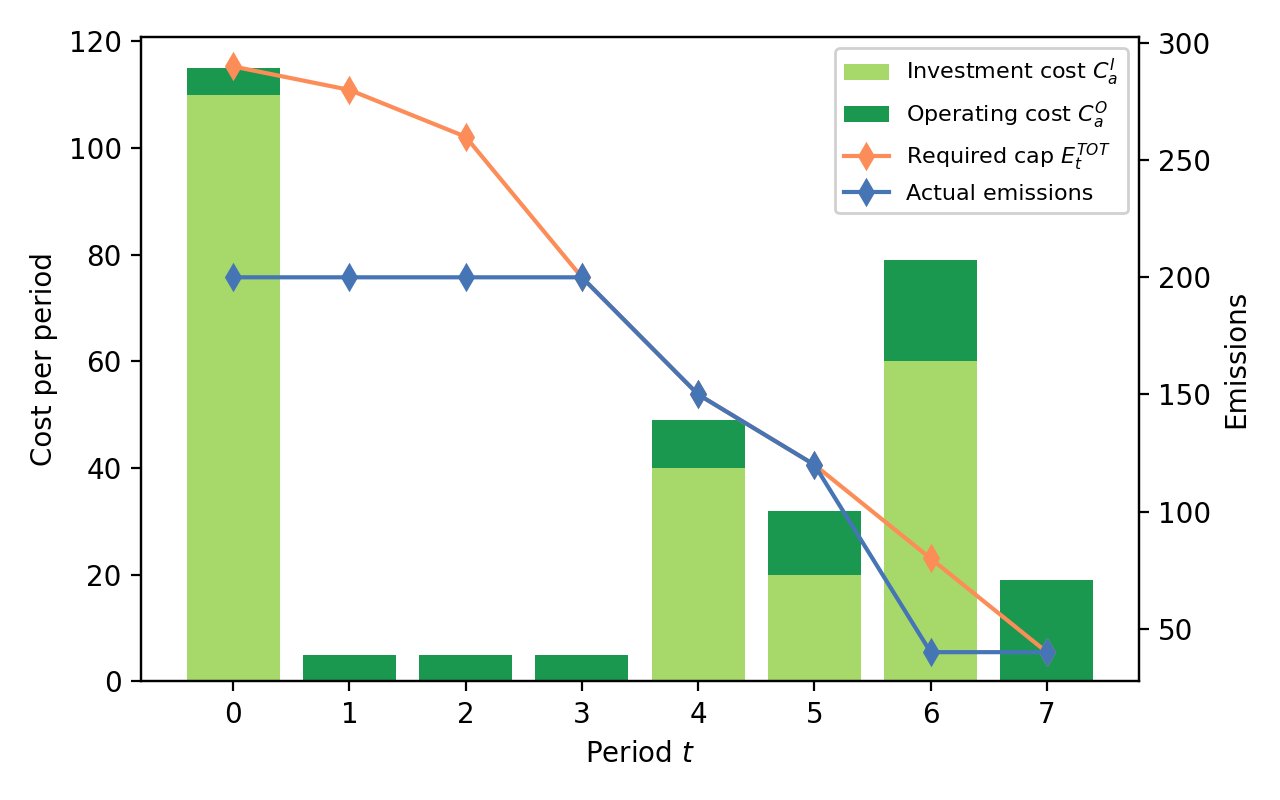
\includegraphics[width=0.75\textwidth]{ch_integer_programming/fleet_retrofit_result.png}
\caption{Cost and emissions over the planning horizon for the worked fleet retrofit instance. Bars: investment (light green) and operating cost (dark green). Lines: required cap (orange) and actual fleet emissions (blue).}
\label{fig:fleet-result}
\end{figure}

\section{Comparing maritime decarbonization regulations: CII, EU ETS, and FuelEU Maritime}
\label{sec:regimes}

To make the situation slightly more complex, a shipowner faces several regulatory instruments at the same time, each with a 
different underlying principle and structure. Here we will focus on three
regulatory instruments that currently applies (from a European perspective): the IMO's Carbon Intensity Indicator (CII), the EU
Emissions Trading System (EU ETS) as extended to shipping, and FuelEU
Maritime itself. Each measures something different, on a different
emissions basis, and enforces itself through a different mechanism.
Understanding that difference is
the point of this section. We will discuss and build each regiulatory regime's model separately.

\subsection{Three different regulatory logics}
\label{sec:regimes-logics}

Table~\ref{tab:regime-comparison} summarises the three instruments along
the dimensions that matter for modelling them: what they measure, on
which emissions basis, and how non-compliance is enforced.

\begin{table}[htbp]
\centering
\caption{Three overlapping maritime decarbonization instruments.}
\label{tab:regime-comparison}
\begin{tabular}{@{}p{0.14\textwidth}p{0.24\textwidth}p{0.16\textwidth}p{0.34\textwidth}@{}}
\toprule
Instrument & What it measures & Basis & Enforcement \\
\midrule
CII & CO2 per unit of transport work (an \emph{efficiency} metric) & Tank-to-wake (TtW) & Letter rating (A--E); rating-based operational and commercial consequences, no direct fine \\
EU ETS & Total CO2 emitted (an \emph{absolute} quantity) & Tank-to-wake (TtW) & Carbon price paid on every tonne, phased in \\
FuelEU Maritime & GHG intensity of energy used (an \emph{intensity} metric) & Well-to-wake (WtW) & Fixed penalty rate on any shortfall against a tightening target \\
\bottomrule
\end{tabular}
\end{table}

The \textit{Basis} is important to take into account. \emph{Tank-to-wake} (TtW)
counts only the CO2 released when the fuel is burned onboard.
\emph{Well-to-wake} (WtW) additionally includes the emissions from
producing and transporting the fuel before it reaches the ship. This is important. FOr instance, 
the CO2 released when burning a biogenic fuel such as
bio-methanol is counted as zero at the tank-to-wake stage, since that
carbon was recently absorbed from the atmosphere by the feedstock; it is
only the WtW basis that carries the fuel's production-stage footprint. A
fuel switch that looks like a complete solution under a TtW-based regime
can therefore be only a partial one under a WtW-based regime. A
second difference is structural rather than accounting-based: CII and
FuelEU both compare an attained value against a target and act only on
the shortfall, while EU ETS charges for every tonne regardless of any
target at all.

\subsection{A very simplified model for illustration}
\label{sec:regimes-setting}

For the regulatory comparison we consider only a single representative
vessel rather than a fleet, choosing a blend of two fuels each period: the incumbent HFO, and
bio-methanol.

\medskip
\noindent\textbf{Sets}: $K=\{\text{HFO},\text{bio}\}$, candidate fuels.

\medskip
\noindent\textbf{Parameters}
\begin{align*}
  Q &&& \text{the vessel's annual energy consumption (GJ), fixed} \\
  TW &&& \text{the vessel's annual transport work (tonne-nautical miles), fixed} \\
  g_k^{\text{TtW}} &&& \text{tank-to-wake CO2 intensity of fuel } k \text{ (gCO2/MJ)} \\
  g_k^{\text{WtW}} &&& \text{well-to-wake GHG intensity of fuel } k \text{ (gCO2e/MJ)} \\
  c_k &&& \text{cost of fuel } k \text{ (EUR/GJ)}
\end{align*}

\noindent\textbf{Core variable}, shared by every model in this section:
\begin{align*}
  x_{kt}\in[0,1] &&& \text{share of energy met by fuel } k \text{ in period } t, \quad \sum_{k\in K}x_{kt}=1.
\end{align*}

Table~\ref{tab:regime-fuels} gives the data used throughout. HFO's TtW
value follows from IMO Annex VI's carbon factor for heavy fuel oil
($C_F=3.114$~gCO2/g fuel) and a representative lower heating value; its
WtW value is FuelEU's own reference intensity, so the difference between
the two ($13.7$~gCO2/MJ) is HFO's upstream, well-to-tank footprint.
Bio-methanol's TtW value is zero under the biogenic-carbon convention
just described; its WtW value of $32.2$~gCO2e/MJ is the production-stage
footprint reported by \citet{cho2027}. Fuel costs are illustrative.

\begin{table}[htbp]
\centering
\caption{Fuel data used throughout this section.}
\label{tab:regime-fuels}
\begin{tabular}{@{}lccc@{}}
\toprule
Fuel & $g_k^{\text{TtW}}$ (gCO2/MJ) & $g_k^{\text{WtW}}$ (gCO2e/MJ) & $c_k$ (EUR/GJ) \\
\midrule
HFO & 77.4 & 91.16 & 15 \\
Bio-methanol & 0.0 & 32.2 & 38 \\
\bottomrule
\end{tabular}
\end{table}

The vessel consumes $Q=10{,}000$~GJ/yr and produces
$TW=75{,}000{,}000$~tonne-nautical miles/yr, giving it a tank-to-wake
attained CII of $77.4\times Q\times1000/TW=10.32$~gCO2/tonne-nm and total
TtW emissions of $774$~tonnes CO2/yr while burning pure HFO --- the
common starting point for every sub-model below.

\subsection{The Carbon Intensity Indicator (CII)}
\label{sec:regimes-cii}

CII compares a vessel's attained carbon intensity,
$\sum_k g_k^{\text{TtW}}x_{kt}\,Q\,1000/TW$ (gCO2/tonne-nm), against a
required value that tightens each year by a fixed reduction factor $r_t$
off a 2019 reference intensity $I^{\text{CII}}_{\text{ref}}$. In
practice a vessel that misses its required value receives a worse letter
rating (D or E) and must file a corrective action plan; there is no
direct fine. We model the commercial consequence of a worse rating, such as
higher financing or insurance cost, a weaker position when chartering, as a 
cost $c^{\text{CII}}$ per tonne of the implied shortfall, making
clear that this is a modelled proxy for an indirect consequence, not a
regulatory payment. In a comprehensive model, the CII may be modelled simply as 
constraints that partly reflects the requirements, and partly company policy/strategy.

\begin{align}
  \min \quad & \sum_{k\in K}c_kx_{kt}\,Q + c^{\text{CII}}s_t^{\text{CII}} \notag\\
  \text{s.t.} \quad & s_t^{\text{CII}} \geq \left(\sum_{k\in K}g_k^{\text{TtW}}x_{kt}\,\frac{Q}{1000} - I^{\text{CII}}_t\,\frac{TW}{10^6}\right), \notag\\
  & \qquad I^{\text{CII}}_t = I^{\text{CII}}_{\text{ref}}(1-r_t) \notag\\
  & \sum_{k\in K}x_{kt}=1, \quad x_{kt}\geq0,\ s_t^{\text{CII}}\geq0. \notag
\end{align}

Using $I^{\text{CII}}_{\text{ref}}=10$~gCO2/tonne-nm and the IMO's
confirmed reduction factors (Table~\ref{tab:cii-factors}), solving this
for each of 2023--2026 gives $x_{\text{bio},t}=0$ throughout, at a
soft-consequence rate of $c^{\text{CII}}=50$~EUR/tonne: the extra fuel
cost of a full switch (EUR~230{,}000/yr) far exceeds even the largest
possible rating consequence (at most
$774\times50=$~EUR~38{,}700/yr, reached only if the required value fell
to zero). A rational owner, at this consequence rate, would simply
accept the worse rating and file the paperwork.

\begin{table}[htbp]
\centering
\caption{IMO CII reduction factors and implied required intensity (illustrative reference intensity of 10 gCO2/tonne-nm).}
\label{tab:cii-factors}
\begin{tabular}{@{}ccc@{}}
\toprule
Year & Reduction factor $r_t$ & Required CII (gCO2/tonne-nm) \\
\midrule
2023 & 5\% & 9.50 \\
2024 & 7\% & 9.30 \\
2025 & 9\% & 9.10 \\
2026 & 11\% & 8.90 \\
\bottomrule
\end{tabular}
\end{table}

\subsection{The EU Emissions Trading System (EU ETS)}
\label{sec:regimes-ets}

EU ETS is structurally simpler: there is no target and no rating, only a
price $c^{\text{CO2}}$ paid on every tonne of TtW CO2 emitted, phased in
at a fraction $\phi_t$ of full scope (Table~\ref{tab:ets-phasein}).

\begin{align}
  \min \quad & \sum_{k\in K}c_kx_{kt}\,Q + \phi_t\,c^{\text{CO2}}\sum_{k\in K}g_k^{\text{TtW}}x_{kt}\,\frac{Q}{1000} \notag\\
  \text{s.t.} \quad & \sum_{k\in K}x_{kt}=1, \quad x_{kt}\geq0. \notag
\end{align}

\begin{table}[htbp]
\centering
\caption{EU ETS phase-in for shipping.}
\label{tab:ets-phasein}
\begin{tabular}{@{}ccc@{}}
\toprule
2024 & 2025 & 2026 onward \\
\midrule
40\% & 70\% & 100\% \\
\bottomrule
\end{tabular}
\end{table}

At today's allowance price of roughly $c^{\text{CO2}}=80$~EUR/tonne,
solving this gives $x_{\text{bio},t}=0$ in every period too: the price
needed to make a full switch worthwhile is, mechanically,
$230{,}000/774\approx297$~EUR/tonne --- almost four times today's price
--- and this threshold is the \emph{same} number that appeared in the
CII sub-model, because both instruments price the same TtW quantity, and
switching fuel changes that quantity the same way regardless of which
instrument is doing the pricing. What differs between the two regimes is
not the price needed to trigger switching, but how much of the vessel's
emissions get priced at all once that threshold is reached: EU ETS
prices every tonne, all the time; CII only prices the shortfall against
a rating.

\subsection{FuelEU Maritime}
\label{sec:regimes-fueleu}

FuelEU compares WtW intensity, not TtW, against its own target
(Table~\ref{tab:fueleu-target-recap}), and its shortfall is priced at a
fixed, deliberately punitive rate --- this is the baseline model of
Section~\ref{sec:fleet-model-v1}, applied to a single vessel:

\begin{align}
  \min \quad & \sum_{k\in K}c_kx_{kt}\,Q + c^{\text{pen}}s_t^{\text{FuelEU}} \notag\\
  \text{s.t.} \quad & s_t^{\text{FuelEU}} \geq \left(\sum_{k\in K}g_k^{\text{WtW}}x_{kt} - I_t^{\text{tar}}\right)\frac{Q}{1000}, \notag\\
  & \sum_{k\in K}x_{kt}=1, \quad x_{kt}\geq0,\ s_t^{\text{FuelEU}}\geq0. \notag
\end{align}

\begin{table}[htbp]
\centering
\caption{FuelEU Maritime target WtW GHG intensity by milestone year.}
\label{tab:fueleu-target-recap}
\begin{tabular}{@{}cccccccc@{}}
\toprule
Year & 2025 & 2030 & 2035 & 2040 & 2045 & 2050 \\
\midrule
$I_t^{\text{tar}}$ (gCO2e/MJ) & 89.34 & 85.69 & 77.95 & 62.90 & 34.64 & 18.23 \\
\bottomrule
\end{tabular}
\end{table}

At $c^{\text{pen}}=700$~EUR/tonne --- well above the 297--390~EUR/tonne
range needed to make switching worthwhile on either basis --- this
regime, and only this one, drives genuine, gradual switching on its own,
shown in Table~\ref{tab:fueleu-solo-recap}: from a token 3\% blend in
2025 to full bio-methanol by 2050, at which point a residual deficit
remains, because bio-methanol's WtW intensity (32.2) still exceeds the
2050 target (18.23). This is exactly the FuelEU behaviour reported in
Section~\ref{sec:fleet-retrofit}, now for a single vessel instead of a
fleet.

\begin{table}[htbp]
\centering
\caption{FuelEU-only optimal bio-methanol share.}
\label{tab:fueleu-solo-recap}
\begin{tabular}{@{}ccccccc@{}}
\toprule
Year & 2025 & 2030 & 2035 & 2040 & 2045 & 2050 \\
\midrule
Bio-methanol share & 3.1\% & 9.3\% & 22.4\% & 47.9\% & 95.9\% & 100\% \\
\bottomrule
\end{tabular}
\end{table}

\subsection{A shipowner facing all three: the combined model}
\label{sec:regimes-combined}

None of the three regimes is optional, so the model a shipowner actually
needs combines all three cost terms over the same fuel choice:

\begin{align}
  \min \quad & \sum_{k\in K}c_kx_{kt}\,Q
    + c^{\text{CII}}s_t^{\text{CII}}
    + \phi_t\,c^{\text{CO2}}\sum_{k\in K}g_k^{\text{TtW}}x_{kt}\,\frac{Q}{1000}
    + c^{\text{pen}}s_t^{\text{FuelEU}} \notag\\
  \text{s.t.} \quad & s_t^{\text{CII}} \geq \left(\sum_{k\in K}g_k^{\text{TtW}}x_{kt}\,\frac{Q}{1000} - I^{\text{CII}}_t\,\frac{TW}{10^6}\right) \notag\\
  & s_t^{\text{FuelEU}} \geq \left(\sum_{k\in K}g_k^{\text{WtW}}x_{kt} - I_t^{\text{tar}}\right)\frac{Q}{1000} \notag\\
  & \sum_{k\in K}x_{kt}=1, \quad x_{kt}\geq0,\ s_t^{\text{CII}},s_t^{\text{FuelEU}}\geq0. \notag
\end{align}

Nothing here is new modelling machinery --- it is literally the union of
the three constraint sets above, added to one objective --- which is the
point: once each regime has its own clean model, combining them is
bookkeeping, not new theory. Solving it, using an illustrative
extrapolation of the CII reduction factor beyond 2026 consistent with
the IMO's 2023 GHG Strategy checkpoints (at least 20\% by 2030, 70\% by
2040, net-zero by 2050, relative to a 2008 reference; ship-specific
factors beyond 2026 have not actually been set), gives the bio-methanol
share in Table~\ref{tab:fueleu-solo-recap} again, \emph{unchanged}, in
every period.

That is a real finding, not a modelling coincidence, and worth
explaining rather than just reporting. Section~\ref{sec:regimes-ets}
already showed that CII and EU ETS, at realistic price levels, cannot
justify switching on their own; adding their costs on top of FuelEU
changes the bill, not the strategy, because FuelEU's own 700~EUR/tonne
rate is already high enough to be the sole driver of the fuel choice ---
CII and EU ETS mostly come along for the ride. They are not free riders,
though: Figure~\ref{fig:regime-comparison} plots the fuel strategy each
regime would choose in isolation, and Table~\ref{tab:regime-cost}
prices out what it would cost to actually \emph{follow} the CII/EU
ETS-optimal strategy (pure HFO, since neither justifies switching alone)
once all three regulations' bills come due on it, against the true joint
optimum.

\begin{figure}[htbp]
\centering
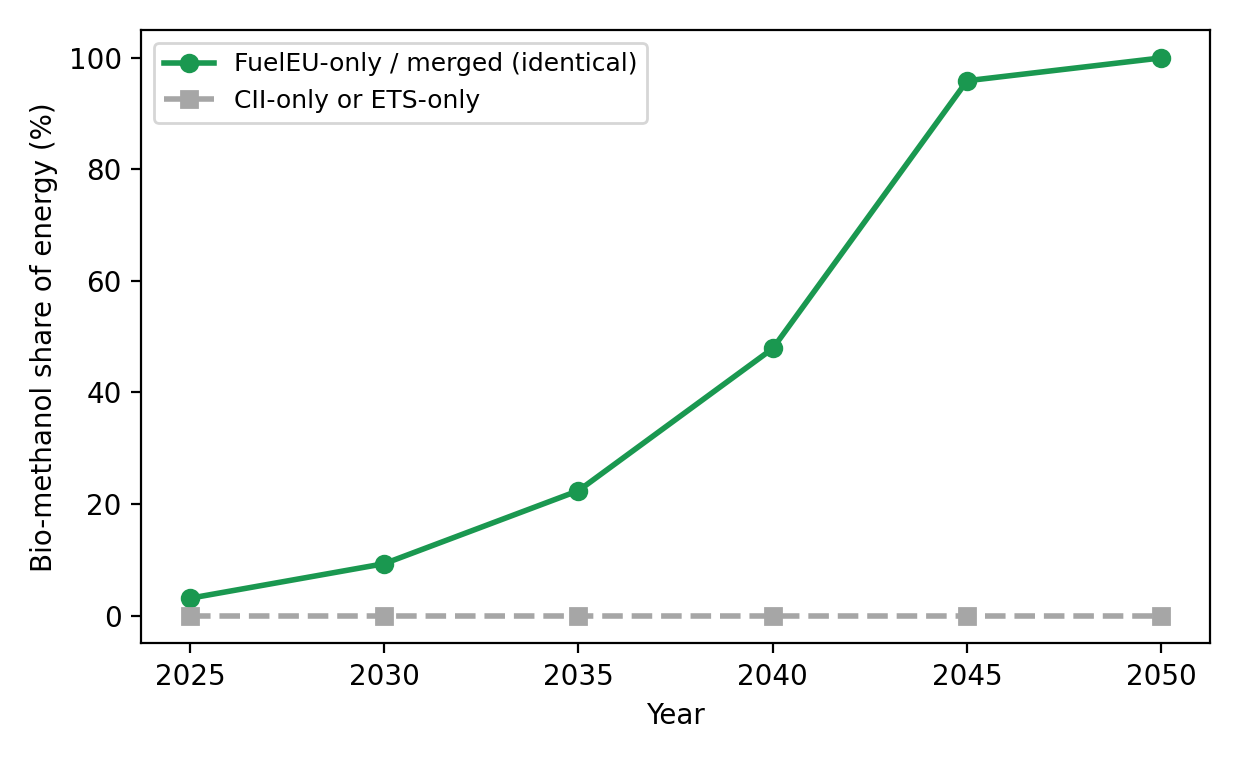
\includegraphics[width=0.7\textwidth]{ch_integer_programming/regime_comparison.png}
\caption{Optimal bio-methanol share under each regime considered in isolation.}
\label{fig:regime-comparison}
\end{figure}

\begin{table}[htbp]
\centering
\caption{Total 2025--2050 cost under the three regulations, by strategy.}
\label{tab:regime-cost}
\begin{tabular}{@{}lr@{}}
\toprule
Strategy & Total cost (EUR) \\
\midrule
Pure HFO (the CII- and EU ETS-optimal choice) & 2{,}629{,}114 \\
Joint optimum (identical to the FuelEU-only strategy) & 1{,}844{,}434 \\
\bottomrule
\end{tabular}
\end{table}

Optimizing only for the two regimes that, individually, never justify
switching costs an extra EUR~785{,}000 over the horizon --- a
43\% premium --- once FuelEU's bill for the same choice is added in. The
general lesson is not ``switch fuels''; it is that a shipowner facing
several overlapping regulations needs to identify which one is actually
\emph{binding} the strategy (here, FuelEU, by design: its rate was set
well above prevailing carbon prices specifically so it would not need
the other two to work) and which are along for the ride, rather than
optimizing against each in isolation and hoping they add up.

The other half of the lesson is the one flagged in
Section~\ref{sec:regimes-logics}: a shipowner who tracked \emph{only}
CII and EU ETS could reasonably conclude that a full switch to
bio-methanol solves everything, since it drives tank-to-wake emissions
to zero. Table~\ref{tab:fueleu-solo-recap} shows that this is not true
under FuelEU: the same fuel, evaluated on a well-to-wake basis, leaves a
persistent shortfall from 2050 onward. Three different regulations,
looking at the same ship and the same fuel, can reach three different
verdicts on how well it is doing --- and a strategy built for one basis
is not automatically a strategy for the others.

Two extensions are natural from here, both left as exercises rather than
developed further. First, FuelEU's own intertemporal flexibility ---
banking a surplus, borrowing against a future one, or pooling compliance
across a fleet's vessels --- can be layered onto its sub-model above
using exactly the constructs of Table~\ref{tab:binary-constructs};
neither CII nor EU ETS, as modelled here, has anything to bank, since
neither carries a balance from one period to the next. Second, CII's
denominator, transport work, has so far been held fixed; the production-function
framework used for ship size and speed earlier in this course is exactly the tool
needed to let speed --- and hence both fuel consumption and transport work
simultaneously --- become a decision variable instead of a parameter,
coupling CII compliance directly to the speed-and-size problem this
course opened with.



% % ch_nlp.tex  —  stub
% Replace this with chapter content

% % ch_uncertainty.tex  —  stub
% Replace this with chapter content

% ch_facility_location.tex  --  Chapter: Facility location and network design
% Part of the TMR4115 compendium. Chapter content only; preamble lives in main.tex.
% Sections 'Single vessel and single charging station' onwards follow
% Agersborg (NTNU MSc thesis, 2025); figures in fig/ch_facility_location/.

\chapter{Facility location and network design}
\label{ch:fl}

In recent years, we have seen how the emission reduction problem for shipping has moved from being primarily a single ship problem, to be a fleet-level problem (especially with FuelEU), and now increasingly also including the design and operation of infrastructure such as ports, bunkering facilities and charging stations. For instance, a methanol dual-fuel vessel is of little use if methanol cannot be bunkered in the ports the vessel visits, and a battery-electric vessel is constrained by where, and how fast, it can recharge. Deciding where to place bunkering hubs, shore-power connections and offshore charging stations is therefore a design decision at the level of the transport system. These decisions interact closely with fleet- and vessel-level design and operational decisions. E.g. the fewer and more distant the energy supply points, the larger the tanks or batteries each vessel must carry.

This chapter introduces the \emph{facility location problem} underpinning these decisions. This is basically a network optimisation problem, thus we start with a basic vocabulary for network models. We then build up the classical location models step by step based on a simple example about the placement of green-fuel bunkering hubs in the North Sea. We then look at a problem related to the placement of offshore charging stations for battery-electric short-sea vessels. This latter case is based on a reformulation of the MSc thesis of \citet{Agersborg2025}.

The learning goals of the chapter are:
\begin{itemize}
  \item Recognise a location problem in a maritime context.
  \item Choose between covering, median, center and fixed-charge objectives.
  \item Formulate the corresponding integer programs.
  \item Explain why some formulations solve much faster than others.
  \item Extend the basic models to cases where the facilities serve moving vessels with limited range (i.e. battery-electric vessels).
\end{itemize}


% ---------------------------------------------------------------------
\section{Networks: a minimal vocabulary}
\label{sec:fl-networks}

A \emph{network} (or graph) $G=(\mathcal{N},\mathcal{A})$ consists of a set of \emph{nodes} $\mathcal{N}$ and a set of \emph{arcs} $\mathcal{A}\subseteq\mathcal{N}\times\mathcal{N}$ connecting pairs of nodes. In maritime applications, nodes typically represent ports, terminals, offshore installations or waypoints, while arcs represent sailing legs, pipelines or cable connections. An arc $(i,j)$ is \emph{directed} if flow may only pass from $i$ to $j$; an undirected \emph{edge} allows flow in both directions and can always be replaced by two opposing arcs. A connected sequence of arcs is a \emph{path}, and a path that returns to its starting node is a \emph{cycle}. Each arc may carry attributes such as a length $D_{ij}$, a unit cost $c_{ij}$ and a capacity $u_{ij}$.

The quantity we move through a network, whether cargo, vessels or energy, is called \emph{flow}, and we denote the flow on arc $(i,j)$ by $x_{ij}$. Nodes are classified by their net flow: in \emph{supply nodes} (sources) flow enters the network, in \emph{demand nodes} (sinks) flow is leaving or beiing absorbed, while in \emph{transshipment nodes} flow is passed on. The fundamental relation that ties a network model together is \emph{flow conservation},
\begin{equation}
  \sum_{j:(i,j)\in\mathcal{A}} x_{ij} \;-\; \sum_{k:(k,i)\in\mathcal{A}} x_{ki} \;=\; b_i
  \qquad \forall i\in\mathcal{N},
  \label{eq:fl-flowcons}
\end{equation}
where $b_i>0$ for supply nodes, $b_i<0$ for demand nodes and $b_i=0$ for transshipment nodes. Put simply: what leaves a node minus what enters it equals what the node itself produces.

Network optimisation problems fall into two categories \citep{Lundgren2010}. In \emph{network flow problems}, the network is given and the question is how to use it: which route a vessel should take (the shortest path problem), how much can be moved from a source to a sink (the maximum flow problem), or how to distribute supply to demand at minimum cost (the minimum cost flow problem, of which the transportation problem is a special case). In \emph{network design problems}, the network itself is the decision: we select which nodes and arcs to establish, typically at a fixed cost, and then use the resulting network. Facility location is the node-selection variant of network design. This chapter concentrates on design; the efficient use of a given network is the topic of a later chapter.

\begin{figure}[htbp]
\centering
\begin{minipage}[b]{0.46\textwidth}
\centering
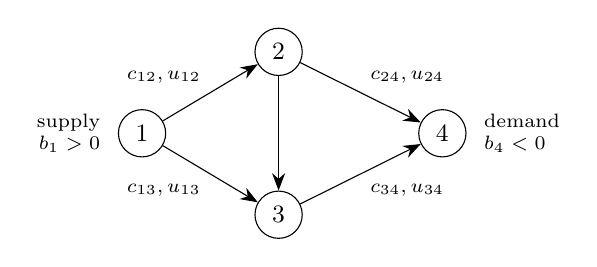
\begin{tikzpicture}[>={Stealth[length=2.2mm]}, node distance=1.6cm,
  nd/.style={circle,draw,minimum size=6mm,inner sep=0pt,font=\small}]
  \node[nd] (1) {1};
  \node[nd, above right=0.6cm and 1.3cm of 1] (2) {2};
  \node[nd, below right=0.6cm and 1.3cm of 1] (3) {3};
  \node[nd, right=3.2cm of 1] (4) {4};
  \draw[->] (1) -- node[above left, font=\scriptsize]{$c_{12},u_{12}$} (2);
  \draw[->] (1) -- node[below left, font=\scriptsize]{$c_{13},u_{13}$} (3);
  \draw[->] (2) -- (3);
  \draw[->] (2) -- node[above right, font=\scriptsize]{$c_{24},u_{24}$} (4);
  \draw[->] (3) -- node[below right, font=\scriptsize]{$c_{34},u_{34}$} (4);
  \node[left=0.1cm of 1, font=\scriptsize, align=right] {supply\\$b_1>0$};
  \node[right=0.1cm of 4, font=\scriptsize, align=left] {demand\\$b_4<0$};
\end{tikzpicture}\\[1mm]
{\small (a) A network flow problem: the network is given.}
\end{minipage}\hfill
\begin{minipage}[b]{0.50\textwidth}
\centering
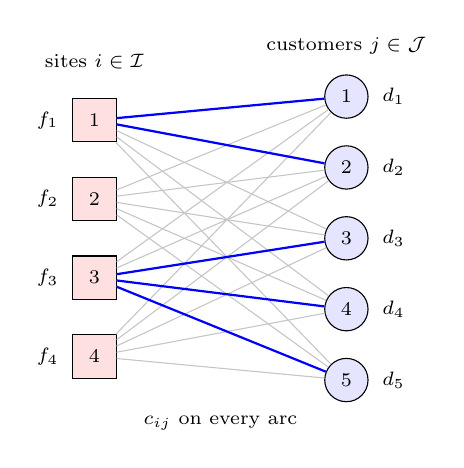
\begin{tikzpicture}[
  fac/.style={rectangle,draw,minimum size=5.5mm,inner sep=0pt,font=\scriptsize,fill=red!12},
  cus/.style={circle,draw,minimum size=5.5mm,inner sep=0pt,font=\scriptsize,fill=blue!10}]
  \foreach \i/\y in {1/1.5,2/0.5,3/-0.5,4/-1.5} {\node[fac] (f\i) at (0,\y) {$\i$};
     \node[left=0.05cm of f\i, font=\scriptsize] {$f_{\i}$};}
  \foreach \j/\y in {1/1.8,2/0.9,3/0,4/-0.9,5/-1.8} {\node[cus] (c\j) at (3.2,\y) {$\j$};
     \node[right=0.05cm of c\j, font=\scriptsize] {$d_{\j}$};}
  \foreach \i in {1,2,3,4} \foreach \j in {1,2,3,4,5} \draw[gray!45] (f\i) -- (c\j);
  \draw[thick,blue] (f1) -- (c1); \draw[thick,blue] (f1) -- (c2);
  \draw[thick,blue] (f3) -- (c3); \draw[thick,blue] (f3) -- (c4); \draw[thick,blue] (f3) -- (c5);
  \node[font=\scriptsize] at (0,2.25) {sites $i\in\mathcal{I}$};
  \node[font=\scriptsize] at (3.2,2.45) {customers $j\in\mathcal{J}$};
  \node[font=\scriptsize] at (1.6,-2.35) {$c_{ij}$ on every arc};
\end{tikzpicture}\\[1mm]
{\small (b) A facility location problem: which sites to open?}
\end{minipage}
\caption{The two families of network problems. In (b), opening site $i$ costs $f_i$, and customers can only be served from open sites; the bold arcs show one possible design with sites 1 and 3 open.}
\label{fig:fl-networks}
\end{figure}

Figure~\ref{fig:fl-networks}(b) shows the structure we will work with throughout the chapter: a bipartite (twosided) network with a set $\mathcal{I}$ of candidate sites on one side and a set $\mathcal{J}$ of customers on the other. If every site were already open, this would be exactly the transportation problem (which is a separate chapter/topic in this course): ship the demand from sites to customers at minimum cost, subject to supply limits. Facility location adds a layer on top, namely a binary decision $y_i$ for each site, and this seemingly small addition turns a linear program into an integer program with a very different character.


% ---------------------------------------------------------------------
\section{The basic structure of a location problem}
\label{sec:fl-anatomy}

There are four main parts of a location problem: a set of candidate locations, a set of demands to be served, a measure of the cost or distance between them, and finally some measure for what a good configuration is. The way each of these parts is modelled defines the problem class.

\emph{Where can facilities be placed?} In \emph{continuous} location, a facility can be placed anywhere in the plane, as in the classical Weber problem of finding the point that minimises the weighted sum of distances to a set of customers \citep{Weber1909}. In \emph{discrete} location, a finite set of candidate sites is given in advance. Maritime infrastructure is usually discrete: bunkering terminals need suitable quays, water depth and permits, and offshore charging stations must be attached to existing structures such as wind turbines, substations or oil and gas platforms. There are also many interesting examples of continuous location models, say, a mobile "energy replenishment vessel" such as Ulstein Thor. Still, we often choose to model also these, restricting the locations to for instance a set of map grid points. Discrete models are also the natural setting for integer programming, and they will be focus here.

\emph{Where is the demand?} In most classical models demand is attached to nodes: a port consumes a certain volume of fuel per year and must be supplied from some facility. For vessels that must refuel or recharge \emph{during} a voyage, however, demand is a concequence of tactical or operational choices (such as routing/scheduling/vessel speed), and a facility is only useful if it lies within reach of the route. We will look at the node-based view first and the route-based view in Section~\ref{sec:fl-charging}.

\emph{What is a good configuration?} Four sets of objectives are common:
\begin{itemize}
  \item \emph{Covering} models require, or reward, that each customer lies within a given service distance of an open facility. Say, locating a fuel station for small boats within 10 nm of cottages with a boat.
  \item \emph{Median} (minisum) models minimise the total demand-weighted distance or transport cost, and thus express efficiency.
  \item \emph{Center} (minimax) models minimise the largest distance from any customer to its nearest facility, and thus express equity or worst-case service.
  \item \emph{Fixed-charge} models let the number of facilities be decided by the model (endogenously) by trading off investment against operating cost. We will later see this in the charging station location problem.
\end{itemize}

\emph{What other constraints are relevant?} Facilities may have limited capacity, customers may be required to use a single facility (single sourcing) or allowed to split their demand, and the problem may be static or span several periods. Table~\ref{tab:fl-models} summarises the models covered in the following sections.

\begin{table}[htbp]
\centering
\caption{The classical discrete location models covered in this chapter.}
\label{tab:fl-models}
\small
\begin{tabular}{@{}llll@{}}
\toprule
Model & Objective & Facilities & Reference \\
\midrule
Location set covering (LSCP) & min.\ number of facilities & endogenous & \citet{Toregas1971} \\
Maximal covering (MCLP) & max.\ covered demand & fixed, $p$ & \citet{Church1974} \\
$p$-median & min.\ weighted distance & fixed, $p$ & \citet{Hakimi1964} \\
$p$-center & min.\ maximum distance & fixed, $p$ & \citet{Hakimi1964} \\
Uncapacitated FLP (UFLP) & min.\ fixed + transport & endogenous & \citet{Balinski1965} \\
Capacitated FLP (CFLP) & min.\ fixed + transport & endogenous & \citet{Daskin2013} \\
\bottomrule
\end{tabular}
\end{table}

\subsection{Example: green-fuel bunkering hubs in the North Sea}
\label{sec:fl-example}

A consortium of fuel suppliers plans a network of bunkering hubs for a zero-carbon fuel, say e-methanol, serving short-sea traffic in the North Sea. Fuel is delivered from each hub by bunker vessel to ten ports that represent the demand, and six of these ports are candidate hub sites. Table~\ref{tab:fl-data} gives the distances, the annual demand $d_j$ at each port, the annualised fixed cost $f_i$ of establishing a hub and the hub throughput capacity $s_i$. Distances are geodesic distances in nautical miles between the port coordinates used by \citet{Agersborg2025}, rounded to whole miles; they underestimate actual sailing distances where land must be rounded. The unit delivery cost is $c=0.04$\,EUR per tonne and nautical mile, so that the annual cost of serving port $j$ from hub $i$ is
\begin{equation}
  c_{ij} = c\, d_j\, D_{ji} \qquad \text{[kEUR/yr, with $d_j$ in kt/yr and $D_{ji}$ in nm]}.
  \label{eq:fl-cij}
\end{equation}
Demands, fixed costs, capacities and the unit delivery cost are sample values and should not be used as estimates of an actual market.

\begin{table}[htbp]
\centering
\caption{Data for the bunkering hub example. Distances $D_{ji}$ in nautical miles, demand $d_j$ in kt fuel per year, fixed cost $f_i$ in kEUR per year, capacity $s_i$ in kt per year.}
\label{tab:fl-data}
\small
\begin{tabular}{@{}lrrrrrrr@{}}
\toprule
 & & \multicolumn{6}{c}{Candidate hub $i$} \\
\cmidrule(l){3-8}
Port $j$ & $d_j$ & Bergen & Stavanger & Aberdeen & Esbjerg & Rotterdam & Immingham \\
\midrule
Lerwick      &  20 & 194 & 222 & 185 & 417 & 525 & 394 \\
Kirkwall     &  15 & 265 & 270 & 115 & 427 & 488 & 335 \\
Aberdeen     &  60 & 302 & 272 &   0 & 365 & 380 & 220 \\
Newcastle    &  40 & 391 & 336 & 130 & 342 & 273 &  93 \\
Immingham    &  70 & 444 & 377 & 220 & 321 & 188 &   0 \\
Rotterdam    & 150 & 510 & 427 & 380 & 262 &   0 & 188 \\
Esbjerg      &  50 & 312 & 229 & 365 &   0 & 262 & 321 \\
Kristiansand &  30 & 158 &  87 & 331 & 162 & 396 & 387 \\
Stavanger    &  50 &  86 &   0 & 272 & 229 & 427 & 377 \\
Bergen       &  60 &   0 &  86 & 302 & 312 & 510 & 444 \\
\midrule
Fixed cost $f_i$ & & 800 & 800 & 600 & 700 & 1000 & 700 \\
Capacity $s_i$   & & 200 & 200 & 200 & 200 &  200 & 200 \\
\bottomrule
\end{tabular}
\end{table}

Total demand is 545\,kt per year, of which Rotterdam alone accounts for more than a quarter. We will now solve the same instance with six different models. Figure~\ref{fig:fl-hubs} at the end of Section~\ref{sec:fl-fixed} shows all six solutions side by side, and it is worth returning to it as each model is introduced.


% ---------------------------------------------------------------------
\section{Covering models}
\label{sec:fl-covering}

Suppose that a bunker vessel can serve a port only if the port lies within a service radius $R$ of the hub, for instance because of the range of the bunker vessel or a contractual delivery-time guarantee. We can define the coverage parameter as
\begin{equation*}
  a_{ij} =
  \begin{cases}
    1 & \text{if } D_{ji}\le R,\\
    0 & \text{otherwise,}
  \end{cases}
\end{equation*}
so that $\mathcal{I}_j=\{i\in\mathcal{I}: a_{ij}=1\}$ is the set of sites that can cover customer $j$. Further, with the binary variables $y_i=1$ if a hub is opened at site $i$, the \emph{location set covering problem} (LSCP) finds the smallest number of hubs that covers every port:
\begin{align}
  \min\quad & \sum_{i\in\mathcal{I}} y_i \label{eq:fl-lscp-obj}\\
  \text{s.t.}\quad & \sum_{i\in\mathcal{I}} a_{ij}\, y_i \ge 1 && \forall j\in\mathcal{J}, \label{eq:fl-lscp-cover}\\
  & y_i\in\{0,1\} && \forall i\in\mathcal{I}. \nonumber
\end{align}
Constraint \eqref{eq:fl-lscp-cover} states that at least one open hub must lie within reach of each port. The model contains no costs at all, only a service requirement, and it answers the question ``how much infrastructure is needed to provide full coverage?'' If the sites have different costs, the objective is simply replaced by $\sum_i f_i y_i$.

For our instance with $R=250$\,nm, three hubs are needed. The solver returns Stavanger, Aberdeen and Immingham, but replacing Immingham with Rotterdam gives an equally good solution: covering models frequently have many alternative optima because the objective only counts facilities. Increasing the radius to 300\,nm reduces the requirement to two hubs, while $R=200$\,nm requires four. The minimum number of facilities is a step function of the service standard, and a decision maker can use this relation to judge whether a stricter standard is worth the extra infrastructure.

In practice, the budget is often fixed before the service standard is. The \emph{maximal covering location problem} (MCLP) turns the question around: given $p$ facilities, how much demand can be covered? We introduce an auxiliary variable $u_j=1$ if customer $j$ is covered:
\begin{align}
  \max\quad & \sum_{j\in\mathcal{J}} d_j\, u_j \label{eq:fl-mclp-obj}\\
  \text{s.t.}\quad & u_j \le \sum_{i\in\mathcal{I}} a_{ij}\, y_i && \forall j\in\mathcal{J}, \label{eq:fl-mclp-link}\\
  & \sum_{i\in\mathcal{I}} y_i = p, \label{eq:fl-mclp-p}\\
  & y_i\in\{0,1\},\; u_j\in\{0,1\} && \forall i\in\mathcal{I},\ j\in\mathcal{J}. \nonumber
\end{align}
Constraint \eqref{eq:fl-mclp-link} allows $u_j=1$ only if at least one covering site is open. With $R=200$\,nm, a single hub at Immingham covers 260\,kt (48\,\% of demand, namely Newcastle, Immingham and Rotterdam). Two hubs, Bergen and Immingham, cover 420\,kt (77\,\%), and three hubs, adding Aberdeen, cover 495\,kt (91\,\%). Each additional hub adds less coverage than the previous one, a pattern of diminishing returns that is typical but, as we will see later, not guaranteed.

Covering models are attractive because the service standard is easy to communicate. Two main weaknesses are that 1) they are "very" binary - a port at 199\,nm counts as fully covered and a port at 201\,nm as not covered at all, and 2) within the range radius the models are indifferent to how far fuel is actually transported.


% ---------------------------------------------------------------------
\section{Median and center models}
\label{sec:fl-median}

To capture the actual transport effort, we introduce allocation variables $x_{ij}\in[0,1]$, the fraction of customer $j$'s demand served from site $i$. Let the unit cost of transporting one unit of demand from site $i$ to customer $j$ be $c_{ij}$. The \emph{$p$-median problem} locates $p$ facilities so that either the total transportation cost, or equivalently, demand-weighted distance, \eqref{eq:fl-cij}, is minimised:
\begin{align}
  \min\quad & \sum_{i\in\mathcal{I}}\sum_{j\in\mathcal{J}} c_{ij}\, d_{j} x_{ij} \label{eq:fl-pmed-obj}\\
  \text{s.t.}\quad & \sum_{i\in\mathcal{I}} x_{ij} = 1 && \forall j\in\mathcal{J}, \label{eq:fl-assign}\\
  & x_{ij} \le y_i && \forall i\in\mathcal{I},\ j\in\mathcal{J}, \label{eq:fl-open}\\
  & \sum_{i\in\mathcal{I}} y_i = p, \label{eq:fl-pmed-p}\\
  & x_{ij}\ge 0,\; y_i\in\{0,1\} && \forall i\in\mathcal{I},\ j\in\mathcal{J}. \nonumber
\end{align}
Constraint \eqref{eq:fl-assign} ensures that all demand is served, and \eqref{eq:fl-open} ensures that it is only served from open sites. Notice that $x_{ij}$ can be continuous: with no capacity limits, each customer will automatically be served entirely from its nearest open facility, since splitting demand can never reduce cost. The name comes from the one-dimensional case, where the optimal single facility location on a line is the (weighted) median of the customer locations.

For the case here, the 1-median is Immingham with an annual transport cost of 5\,247\,kEUR. The 2-median is Stavanger and Rotterdam (2\,724\,kEUR), and the 3-median adds Aberdeen (1\,720\,kEUR). Make a note that Immingham, the best single location, is not part of the best pair. Optimal solutions for different $p$ need not be \emph{nested}, and this has a practical consequence if we want to develop a service step-by-step. If we simply start with the best single site and then adds sites one at a time will generally not end up in the best configuration. We will see this again in the charging case.

The median objective rewards serving large demands well, and may leave small, remote customers far from any facility. The \emph{$p$-center problem} instead minimises the worst-case distance $L$ to the nearest facility:
\begin{align}
  \min\quad & L \label{eq:fl-pcen-obj}\\
  \text{s.t.}\quad & \sum_{i\in\mathcal{I}} D_{ji}\, x_{ij} \le L && \forall j\in\mathcal{J}, \label{eq:fl-pcen-L}\\
  & \eqref{eq:fl-assign}, \eqref{eq:fl-open}, \eqref{eq:fl-pmed-p}, \quad x_{ij}\in\{0,1\}. \nonumber
\end{align}
The auxiliary variable $L$ is a standard linearisation of a $\min\max$ objective: minimising a variable that is forced to be at least as large as every term is equivalent to minimising the largest term. Here $x_{ij}$ must be binary, since a fractional assignment would let \eqref{eq:fl-pcen-L} average distances rather than select one. The 2-center for our instance is Stavanger and Immingham, with a maximum distance of 270\,nm (Kirkwall to Stavanger).

Table~\ref{tab:fl-compare} evaluates the three candidate pairs that are optimal under the three different criteria. Each pair wins on its own criterion and loses on at least one other. None of them is ``the'' optimal pair of hubs; the choice of objective \emph{is} a design decision, and it should reflect what the infrastructure is meant to achieve: low total supply cost, a guaranteed maximum delivery distance, or high coverage within a service standard.

\begin{table}[htbp]
\centering
\caption{Three pairs of hubs evaluated under three criteria. Bold entries mark the optimum for each criterion.}
\label{tab:fl-compare}
\small
\begin{tabular}{@{}lrrr@{}}
\toprule
Hubs & Transport cost & Max.\ distance & Demand within 200\,nm \\
 & [kEUR/yr] & [nm] & [kt/yr] \\
\midrule
Stavanger, Rotterdam & \textbf{2\,724} & 273 & 360 \\
Stavanger, Immingham & 2\,913 & \textbf{270} & 400 \\
Bergen, Immingham    & 3\,105 & 312 & \textbf{420} \\
\bottomrule
\end{tabular}
\end{table}


% ---------------------------------------------------------------------
\section{Fixed-charge models}
\label{sec:fl-fixed}

In the models so far, the number of facilities was either the objective (LSCP) or a given parameter $p$. In most investment decisions the number of facilities is itself something to be decided by weighing investment cost against operating cost. The \emph{uncapacitated facility location problem} (UFLP) does this by adding the fixed cost of each open site to the transport cost:
\begin{align}
  \min\quad & \sum_{i\in\mathcal{I}} f_i\, y_i + \sum_{i\in\mathcal{I}}\sum_{j\in\mathcal{J}} c_{ij}\, x_{ij} \label{eq:fl-uflp-obj}\\
  \text{s.t.}\quad & \eqref{eq:fl-assign},\ \eqref{eq:fl-open}, \quad x_{ij}\ge 0,\; y_i\in\{0,1\}. \nonumber
\end{align}
The UFLP is the $p$-median problem with the cardinality constraint \eqref{eq:fl-pmed-p} replaced by a price on each facility. Opening one more hub is worthwhile only if the reduction in transport cost exceeds its fixed cost.

The optimal solution opens Stavanger, Aberdeen and Rotterdam at a total cost of 4\,120\,kEUR per year, of which 2\,400 is fixed cost and 1\,720 transport cost. This is the 3-median configuration found earlier, so in this instance the fixed costs select $p=3$ as the right number of hubs. Stavanger serves the Norwegian and Danish ports (190\,kt), Aberdeen serves the UK ports north of the Humber (135\,kt), and Rotterdam serves itself and Immingham (220\,kt). The solution is sensitive to the level of fixed costs: halving all $f_i$ makes it optimal to open five hubs, while increasing them by 50\,\% reduces the network to two hubs, Stavanger and Immingham.

The UFLP solution loads the Rotterdam hub with 220\,kt per year. If each hub can handle at most $s_i$ per year, we add the capacity constraint
\begin{equation}
  \sum_{j\in\mathcal{J}} d_j\, x_{ij} \le s_i\, y_i \qquad \forall i\in\mathcal{I},
  \label{eq:fl-cap}
\end{equation}
which gives the \emph{capacitated facility location problem} (CFLP). The right-hand side $s_i y_i$ does double duty: it limits the throughput of an open hub and forces the throughput of a closed hub to zero. With $s_i=200$\,kt, the cheapest adjustment keeps the same three hubs and splits Immingham's demand, sending 50\,kt from Rotterdam and 20\,kt from Aberdeen. The total cost increases by only 26\,kEUR to 4\,146\,kEUR, because 20\,kt now travel 220\,nm instead of 188\,nm.

Split deliveries may be operationally unattractive, since each port would have to contract with two suppliers. Requiring \emph{single sourcing}, that is $x_{ij}\in\{0,1\}$, changes the picture. The best single-sourcing assignment to the same three hubs costs 4\,305\,kEUR, and it is now cheaper to open a fourth hub at Immingham, which serves Newcastle and itself. The total cost becomes 4\,235\,kEUR, and the fixed-cost share rises from 58 to 73\,\%. Note that with capacities, the assignment variables are no longer automatically integral, and single sourcing must be enforced explicitly. Figure~\ref{fig:fl-hubs} summarises the six solutions.

\begin{figure}[htbp]
\centering
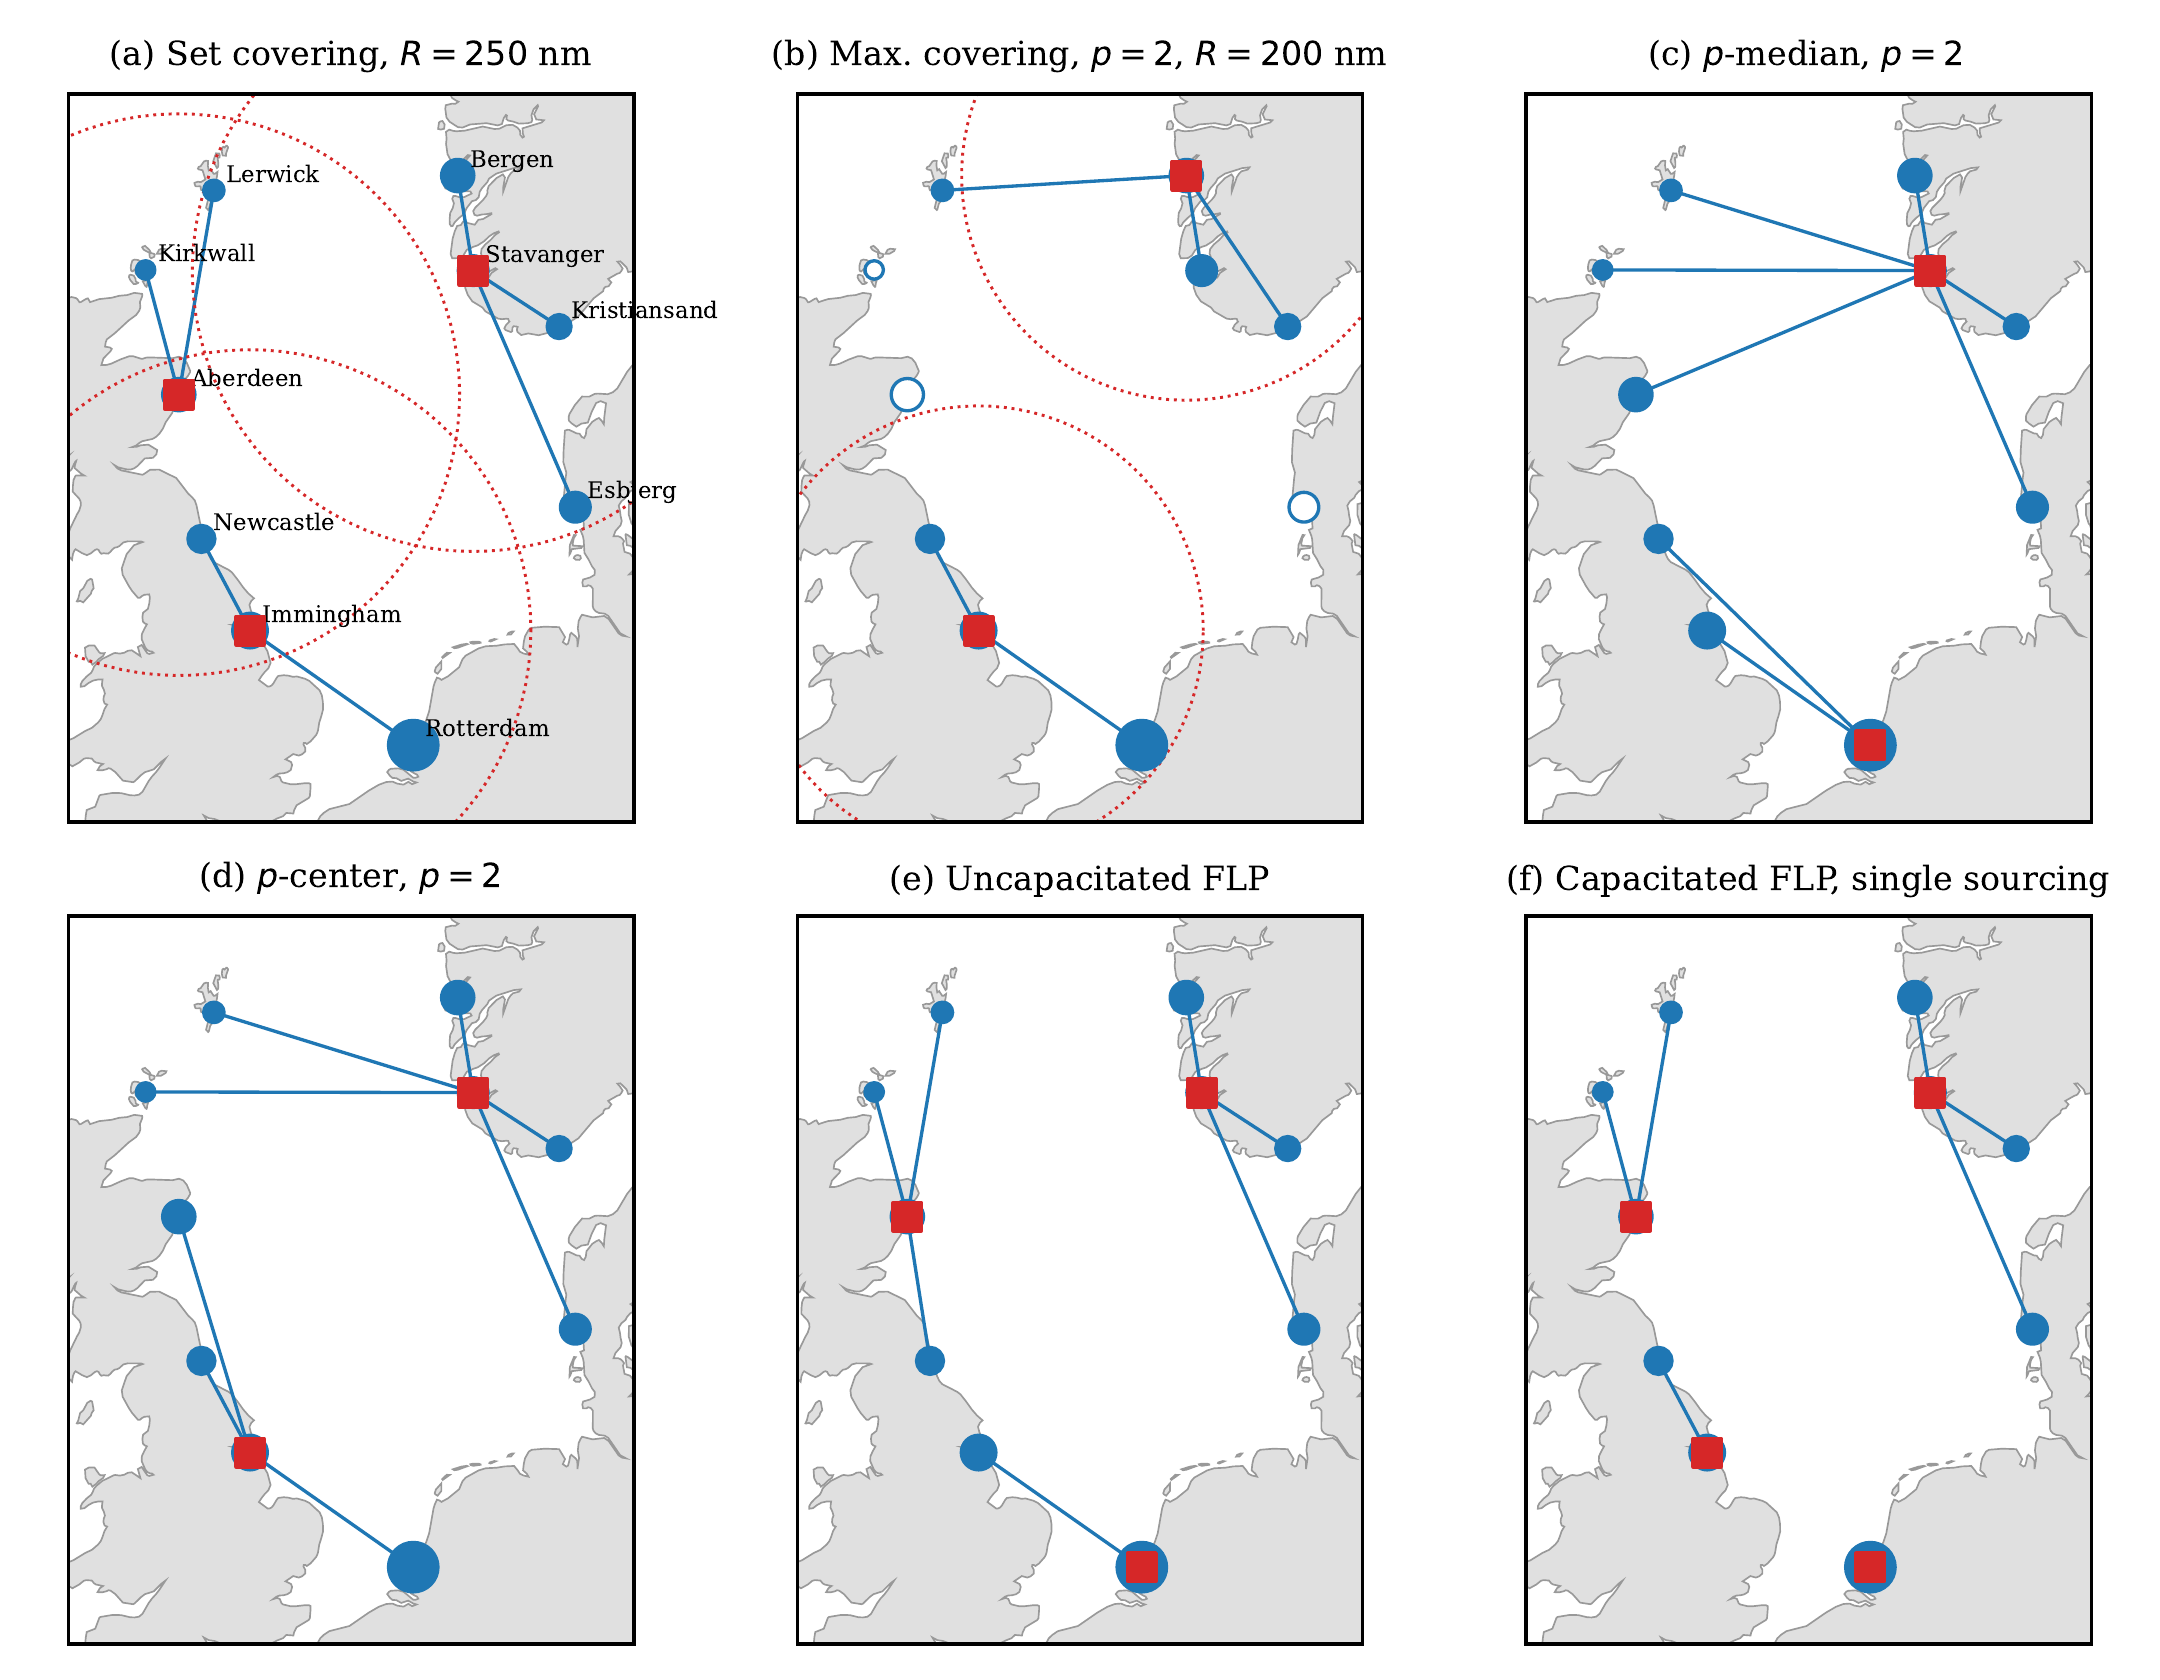
\includegraphics[width=\textwidth]{ch_facility_location/fl_hub_solutions.png}
\caption{Six models, one instance. Red squares are open hubs, circles are ports with area proportional to demand, and lines show assignments. In the covering models (a) and (b), dotted circles show the service radius and open circles are uncovered ports. Straight lines are schematic and do not represent sailing routes.}
\label{fig:fl-hubs}
\end{figure}


% ---------------------------------------------------------------------
\section{Formulation strength (not compulsory reading)}
\label{sec:fl-strength}

The UFLP can be written in a second way. Constraint \eqref{eq:fl-open} contains one inequality for every site--customer pair, $|\mathcal{I}|\times|\mathcal{J}|=60$ constraints in our instance. It is tempting to aggregate them into one constraint per site,
\begin{equation}
  \sum_{j\in\mathcal{J}} x_{ij} \le |\mathcal{J}|\, y_i \qquad \forall i\in\mathcal{I},
  \label{eq:fl-weak}
\end{equation}
which is also valid: if $y_i=0$ no customer can be served from $i$, and if $y_i=1$ the constraint is redundant. Both formulations have exactly the same integer solutions, and the aggregated version needs only six constraints. Which one is better?

Recall from the chapter on integer programming that branch-and-bound relies on the linear programming (LP) relaxation to provide bounds. A formulation is \emph{stronger} than another if its LP relaxation is tighter, that is, closer to the convex hull of the integer solutions. Relaxing $y_i\in\{0,1\}$ to $0\le y_i\le 1$ in our instance gives the following results. With the disaggregated constraints \eqref{eq:fl-open}, the LP relaxation returns $4\,120$\,kEUR with all $y_i$ integral, so the integer optimum is found without any branching. With the aggregated constraints \eqref{eq:fl-weak}, the LP relaxation returns only $1\,200$\,kEUR. Here the LP opens a fraction $y_i=\tfrac{1}{10}\sum_j x_{ij}$ of every site and pays correspondingly little in fixed costs; each hub site serves itself at zero distance, and the remaining ports are served from their nearest site. The resulting gap of 71\,\% must be closed by branching.

The lesson generalises well beyond facility location: fewer constraints does not mean an easier model. A constraint such as $x_{ij}\le y_i$ carries much more information in the LP relaxation than its aggregated counterpart, and for large instances the difference between the two formulations can be the difference between seconds and days of computation. The strong formulation of the UFLP is often attributed to \citet{Balinski1965}; see \citet{Cornuejols1990} for a thorough treatment. The same reasoning applies whenever a ``big-$M$'' constraint links a continuous quantity to a binary decision: $M$ should be as small as the problem allows.


% ---------------------------------------------------------------------
\section{Implementation in Python}
\label{sec:fl-python}

Listing~\ref{lst:fl-xpress} implements the UFLP and CFLP in Xpress Python. As in earlier chapters, the data are kept in separate files and read with pandas, so that the same model code can be used for other instances. The three runs at the end reproduce the UFLP, the CFLP with split deliveries, and the CFLP with single sourcing.

\begin{lstlisting}[language=Python, caption={UFLP and CFLP in Xpress Python.}, label={lst:fl-xpress}]
import pandas as pd
import xpress as xp

# ---- Data --------------------------------------------------------------
dist  = pd.read_csv("distances.csv", index_col="port")   # D_ji [nm]
ports = pd.read_csv("ports.csv", index_col="port")        # d_j [kt/yr]
hubs  = pd.read_csv("hubs.csv", index_col="hub")          # f_i [kEUR/yr], s_i [kt/yr]
c_unit = 0.04                                             # kEUR per (kt nm)

I, J = list(hubs.index), list(ports.index)
cost = {(i, j): c_unit * ports.demand[j] * dist.loc[j, i] for i in I for j in J}

def solve_flp(capacitated=False, single_sourcing=False):
    m = xp.problem("facility_location")
    y = {i: m.addVariable(vartype=xp.binary, name=f"y_{i}") for i in I}
    xtype = xp.binary if single_sourcing else xp.continuous
    x = {(i, j): m.addVariable(lb=0, ub=1, vartype=xtype, name=f"x_{i}_{j}")
         for i in I for j in J}

    m.setObjective(xp.Sum(hubs.fixed_cost[i] * y[i] for i in I)
                   + xp.Sum(cost[i, j] * x[i, j] for i in I for j in J),
                   sense=xp.minimize)
    m.addConstraint(xp.Sum(x[i, j] for i in I) == 1 for j in J)   # serve all
    m.addConstraint(x[i, j] <= y[i] for i in I for j in J)        # open to use
    if capacitated:
        m.addConstraint(xp.Sum(ports.demand[j] * x[i, j] for j in J)
                        <= hubs.capacity[i] * y[i] for i in I)
    m.controls.outputlog = 0
    m.solve()
    opened = [i for i in I if m.getSolution(y[i]) > 0.5]
    return m.attributes.objval, opened, {k: m.getSolution(v) for k, v in x.items()}

for case in [dict(), dict(capacitated=True),
             dict(capacitated=True, single_sourcing=True)]:
    z, opened, _ = solve_flp(**case)
    print(case, round(z, 1), opened)
\end{lstlisting}

Porting the model to Gurobi requires only the usual substitutions (\texttt{gp.Model}, \texttt{addVar}, \texttt{GRB.BINARY}, \texttt{setObjective}, \texttt{optimize}); the model structure is unchanged.


% ---------------------------------------------------------------------
\section{When the demand travels: offshore charging for battery-electric vessels}
\label{sec:fl-charging}

Green fuels are definitely among the many emission reducton alternatives that must be part of the solution for maritime decarbonisation. However, there are large intrinsic losses resulting from the conversion of (valuable) green electricity to fuels, and then back again to electricity onboard the vessel.  Figure~\ref{fig:fl-fuel-footprint} shows the illustrative fuel and CO$_2$ footprint for a selection of alternative marine fuels, including battery-electric operation. Thus, if we can store and use the electricty directly, without conversion, this is highly preferable from an overall energy efficiency point-of-view.

\begin{figure}[htbp]
\centering
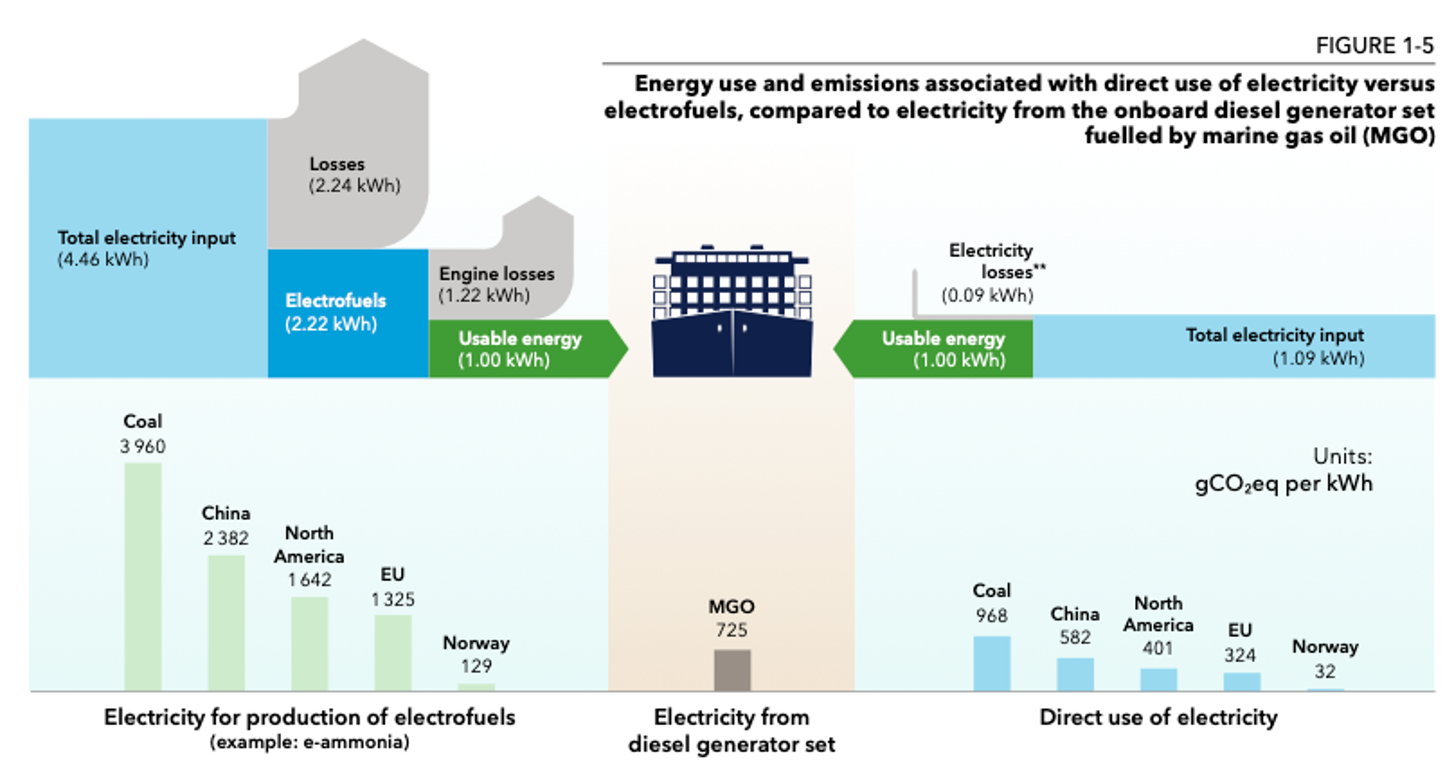
\includegraphics[width=1.00\textwidth]{ch_facility_location/dnv_fuel_co2_footprint.png}
\caption{Illustrative fuel and CO$_2$ footprint comparison for alternative marine fuels.}
\label{fig:fl-fuel-footprint}
\end{figure}

However, the energy density of marine batteries, both by weight and volume, limits the distance a vessel can sail between being recharged, thus excluding routes with long port-to-port distances. One possible solution to this, extending the feasible range of all-electric propulsion, is to locate charging stations offshore. We already have offshore charging stations at wind turbine farms. They are currently installed for the charging SOVs used for wind farm inpection and maintenance, but could with moderate changes in design be repurposed for short sea shipping. Also oil and gas installations have recently been electrified (from the onshore grid). Thus, it is interesting to explore how we could make battery-electric operation feasible on routes that are too long to sail on one charge \citep{Agersborg2025}. Where should such stations be placed?

Two features distinguish this problem from the bunkering hub example. First, demand is not located at nodes. A vessel sailing from Aberdeen to Bergen can manage with a smaller battery if there are one or several charging stations along the route. This is the maritime counterpart of the \emph{flow refuelling location problem}, developed for alternative-fuel stations serving road vehicles with limited range \citep{Hodgson1990, Kuby2005}, where customers are origin--destination flows rather than points. Thus, the infrastructure decision interacts with a vessel design decision. The installed battery capacity $q$ must cover the longest leg between two charging opportunities, and every unit of battery capacity displaces cargo. The location of the stations thus determines the size of the batteries, and the cost of batteries in turn influences where the stations should be.

The problem and model will be developed stepwise (again according to ) \citet{Agersborg2025}). First one vessel and one offshore charging station, then a fleet sharing one station, and finally a fleet with several stations. Candidate sites are the 62 existing and planned offshore wind farms in the North Sea. All parameter values in this section are taken from the illustrative cases of the thesis and are expressed in abstract monetary and energy units.


This section presents multiple iterations of the optimization model developed for determining the optimal placement of offshore charging stations. The models are formulated using MILP and aims to minimize total vessel operational costs. Factors such as vessel energy consumption, sailing distance, loss of cargo space due to batteries and time usage is considered. An illustrative case is provided for each iteration to demonstrate its application and validate the model's results.


% ---------------------------------------------------------------------
\subsection{Single vessel and single charging station}
\label{sec:single-vessel-single-station}

The first iteration of the optimization model simplifies the problem to its most basic form: a single battery-electric vessel traveling between two ports with a mandatory stop at exactly one potential offshore charging station, selected from a predefined set of wind farm locations ($\mathcal{W}$). The primary goal here is to establish the core optimization logic and understand the fundamental trade-offs involved in selecting a single charging station location based on minimizing total voyage costs, considering energy needs and operational factors.

\subsubsection{Model formulation}
\label{sec:single-formulation}

The model is formulated as a MILP. The sets, parameters, and decision variables used in this first iteration are defined in Table~\ref{tab:single-notation}.

\begin{table}[H]
\centering
\caption{Sets, parameters and variables for single vessel and single charging station optimization model.}
\label{tab:single-notation}
\begin{tabular}{@{}ll@{}}
\toprule
\multicolumn{2}{@{}l}{\textbf{Sets}}\\
\midrule
$\mathcal{P}$ & Set of ports (Origin $O$ and destination $D$).\\
$\mathcal{W}$ & Set of potential wind farm locations.\\
$\mathcal{N}$ & Set of all nodes, where $\mathcal{N}=\mathcal{P}\cup\mathcal{W}$ (All nodes).\\
$\mathcal{A}$ & Set of arcs between nodes, where $\mathcal{A}=\{(i,j)\mid i,j\in\mathcal{N},\; i\neq j\}$.\\
\midrule
\multicolumn{2}{@{}l}{\textbf{Parameters}}\\
\midrule
$C^{S}$      & Sailing cost per nautical mile.\\
$E^{C}$      & Energy consumption per nautical mile.\\
$C^{LO}$     & Lost opportunity cost per unit cargo space.\\
$Q$          & Maximum possible battery capacity.\\
$C^{E}_{i}$  & Cost per unit of energy at node $i$.\\
$D_{ij}$     & Geodesic distance between node $i$ and node $j$.\\
$V$          & Sailing speed.\\
$C^{T}$      & Time cost per hour.\\
$R^{C}$      & Charging rate.\\
$M$          & A large constant, e.g.\ $M=|\mathcal{W}|+2$.\\
\midrule
\multicolumn{2}{@{}l}{\textbf{Variables}}\\
\midrule
$q\ge 0$             & Installed battery capacity.\\
$b_{i}\ge 0$         & Battery level when departing node $i$.\\
$x_{i}\ge 0$         & Amount of energy charged at node $i$.\\
$y_{i}\in\{0,1\}$    & 1 if recharging occurs at node $i$, 0 otherwise.\\
$z_{ij}\in\{0,1\}$   & 1 if arc from node $i$ to node $j$ is used, 0 otherwise.\\
\bottomrule
\end{tabular}
\end{table}

\subsubsection*{Objective Function}

The objective function (\ref{eq:obj-single}) aims to minimize the total estimated cost for the single voyage. This cost comprises four key components:

\begin{enumerate}
\item \textbf{Sailing Cost:} Calculated from the total distance traveled along selected segments and the vessel's cost per nautical mile ($C^{S}$).
\item \textbf{Energy Cost:} Representing the expense for energy replenishment, determined by the amount charged ($x_{i}$) and the energy price ($C^{E}_{i}$) at visited nodes.
\item \textbf{Lost Opportunity Cost:} Reflecting the economic impact of dedicating cargo space to the battery system, calculated from the installed battery capacity ($q$) and a cost per unit ($C^{LO}$).
\item \textbf{Time Cost:} Monetizing the overall duration of the voyage, including both sailing and charging time, multiplied by a time-based cost ($C^{T}$) (e.g., charter rate or equivalent operational time expense).
\end{enumerate}

While the sailing cost (distance-based) and time cost (duration-based) can sometimes be difficult to separate in real-world operations, they are included as distinct components in this model to offer greater flexibility. This allows for scenarios where one might be emphasized over the other, for instance if only a pure time-based operational cost is relevant, the sailing cost parameter ($C^{S}$) can simply be set to zero, and vice-versa.

\begin{equation}
\min\;
\underbrace{\sum_{(i,j)\in\mathcal{A}} z_{ij}\,D_{ij}\,C^{S}}_{\text{Sailing cost}}
\;+\;
\underbrace{\sum_{i\in\mathcal{N}} C^{E}_{i}\,x_{i}}_{\text{Energy cost}}
\;+\;
\underbrace{q\,C^{LO}}_{\text{Lost-opportunity cost}}
\;+\;
\underbrace{C^{T}\left(\sum_{(i,j)\in\mathcal{A}} \frac{D_{ij}}{V}\,z_{ij}
      \;+\; \sum_{i\in\mathcal{N}} \frac{x_{i}}{R^{C}}\right)}_{\text{Time cost}}
\label{eq:obj-single}
\end{equation}

Subject to:

\begin{align}
&\sum_{\substack{(i,j)\in\mathcal{A}\\ i=O}} z_{ij} = 1 \label{eq:depart-origin}\\[2pt]
&\sum_{\substack{(i,j)\in\mathcal{A}\\ j=D}} z_{ij} = 1 \label{eq:arrive-dest}\\[2pt]
&\sum_{\substack{(i,j)\in\mathcal{A}\\ i=u}} z_{ij}
 \;-\; \sum_{\substack{(k,i)\in\mathcal{A}\\ i=u}} z_{ki} = 0
 && \forall\, u\in\mathcal{W} \label{eq:flow-cons}\\[2pt]
&q \le Q \label{eq:cap-max}\\[2pt]
&b_{i} \le q && \forall\, i\in\mathcal{W} \label{eq:soc-le-q}\\[2pt]
&b_{O} = q \label{eq:soc-origin}\\[2pt]
&b_{D} = q \label{eq:soc-dest}\\[2pt]
&b_{j} \ge b_{i} - E^{C}D_{ij} + x_{j} - M\!\left(1-z_{ij}\right)
 && \forall\, (i,j)\in\mathcal{A} \label{eq:energy-lo}\\[2pt]
&b_{j} \le b_{i} - E^{C}D_{ij} + x_{j} + M\!\left(1-z_{ij}\right)
 && \forall\, (i,j)\in\mathcal{A} \label{eq:energy-hi}\\[2pt]
&b_{i} \ge E^{C}D_{ij} - M\!\left(1-z_{ij}\right)
 && \forall\, (i,j)\in\mathcal{A} \label{eq:energy-suff}\\[2pt]
&\sum_{(k,i)\in\mathcal{A}} z_{ki} = y_{i} && \forall\, i\in\mathcal{W} \label{eq:visit-link}\\[2pt]
&\sum_{i\in\mathcal{W}} y_{i} = 1 \label{eq:one-station}\\[2pt]
&z_{ij}\in\{0,1\},\quad y_{i}\in\{0,1\},\quad b_{i}\ge 0,\quad x_{i}\ge 0,\quad q\ge 0
 \label{eq:domains}
\end{align}

\subsubsection*{Model Explanation}

The constraints implemented ensure a feasible and logical solution. Route definition constraints (\ref{eq:depart-origin}, \ref{eq:arrive-dest}) ensure the vessel departs the origin $O$ and arrives at the destination $D$ exactly once. Flow conservation through constraints (\ref{eq:flow-cons}) mandates that if the vessel visits a wind farm node ($u\in\mathcal{W}$), it must also depart from it, maintaining route continuity and preventing the voyage from ending prematurely at a charging location.

Energy management is governed by constraints (\ref{eq:cap-max}) through (\ref{eq:energy-suff}). These limit the installed battery capacity $q$ to a maximum $Q$, ensure the battery state $b_{i}$ upon departure never exceeds installed battery capacity $q$, set the battery state at the origin and destination to full capacity, and manage the energy balance between nodes using the ''big-M'' method to account for consumption and charging only on utilized arcs ($z_{ij}=1$). Constraint (\ref{eq:energy-suff}) ensures sufficient energy to reach the next selected node. Charging station assignment is handled by (\ref{eq:visit-link}) and (\ref{eq:one-station}), which link the selection of a node $i$ as the charging station ($y_{i}=1$) to the vessel actually visiting it, while ensuring exactly one wind farm location is chosen overall. Finally, constraint (\ref{eq:domains}) defines the nature of the decision variables (binary, continuous, non-negative).

\subsubsection{Illustrative case}
\label{sec:single-case}

To demonstrate the model's application, the route between Aberdeen and Bergen is chosen as a representative North Sea short-sea shipping route (port details in Table~\ref{tab:single-ports}). Two cost scenarios are analyzed to assess the model's behavior under the parameter values detailed in Table~\ref{tab:single-params}. Scenario 1 has a high lost opportunity cost ($C^{LO}=100$) relative to sailing cost ($C^{S}=10$), while Scenario 2 has a lower lost opportunity cost ($C^{LO}=50$) and higher sailing cost ($C^{S}=20$). All other parameters remain constant between the scenarios.

\begin{table}[H]
\centering
\caption{Set of ports for single vessel illustrative case. Coordinates retrieved from (MagicPort 2025)}
\label{tab:single-ports}
\begin{tabular}{@{}llrr@{}}
\toprule
Port city & Unlocode & Lat & Long \\
\midrule
Aberdeen & GBABD & 57.14 & $-2.08$ \\
Bergen   & NOBGO & 60.39 & 5.32 \\
\bottomrule
\end{tabular}
\end{table}

\begin{table}[H]
\centering
\caption{Parameters for single vessel illustrative case.}
\label{tab:single-params}
\begin{tabular}{@{}lccl@{}}
\toprule
Parameter & Scenario 1 & Scenario 2 & Unit \\
\midrule
$O$          & ABD  & BGO  & -- \\
$D$          & BGO  & ABD  & -- \\
$C^{S}$      & 10   & 20   & per nm \\
$E^{C}$      & 0.2  & 0.2  & per nm \\
$C^{LO}$     & 100  & 50   & per unit cargo space lost \\
$Q$          & 1000 & 1000 & units of cargo space \\
$C^{E}_{w}$  & 10   & 10   & per unit energy \\
$C^{E}_{p}$  & 5    & 5    & per unit energy \\
$V$          & 15   & 15   & knots \\
$C^{T}$      & 0    & 0    & cost per hour \\
$R^{C}$      & 2    & 2    & units per hour \\
\bottomrule
\end{tabular}
\end{table}

\subsubsection*{Model output}

The optimization yields different optimal charging station locations for the two scenarios. Sørvest A is selected for Scenario 1, while Vestavind E is chosen for Scenario 2. The detailed results in Table~\ref{tab:single-results} show that Scenario 1, with its high penalty for battery size, results in a smaller required battery capacity (37.6 units) but necessitates a longer route (345 nm, 114\% of direct distance) via the more centrally located Sørvest A. Scenario 2, prioritizing shorter sailing distance due to its higher cost, justifies installing a larger battery (44.7 units) to enable a more direct route (311 nm, 103\% of direct) by choosing Vestavind E. Figure~\ref{fig:single-routes} illustrates the routes chosen as the optimal solution for the two scenarios, and Figure~\ref{fig:single-soc} illustrates the corresponding battery SOC profiles.

\begin{table}[H]
\centering
\caption{Results for Scenario 1 and Scenario 2}
\label{tab:single-results}
\begin{tabular}{@{}lcc@{}}
\toprule
 & \textbf{Scenario 1} & \textbf{Scenario 2} \\
\midrule
Route                            & GBABD $\rightarrow$ NOBGO & GBABD $\rightarrow$ NOBGO \\
Charging station                 & Sørvest A   & Vestavind E \\
\textbf{Vessel-specific cost}    & \textbf{7703} & \textbf{8848} \\
\quad -- Sailing cost            & 3448 & 6213 \\
\quad -- Lost opportunity cost   & 3752 & 2237 \\
\quad -- Energy cost             & 502  & 398  \\
\quad -- Time cost               & 0    & 0    \\
\textbf{Total time in hours}     & \textbf{57.5} & \textbf{51.8} \\
\quad -- Sailing                 & 23.0 & 20.7 \\
\quad -- Charging in port        & 18.8 & 22.4 \\
\quad -- Charging offshore       & 15.7 & 8.7  \\
Installed battery capacity $q_{v}$ & 37.6 & 44.7 \\
Total distance in nm             & 345  & 311  \\
\% of direct distance            & 114\% & 103\% \\
Longest segment in nm            & 188  & 224  \\
\bottomrule
\end{tabular}
\end{table}

\begin{figure}[H]
\centering
\begin{minipage}[b]{0.48\textwidth}
  \centering
  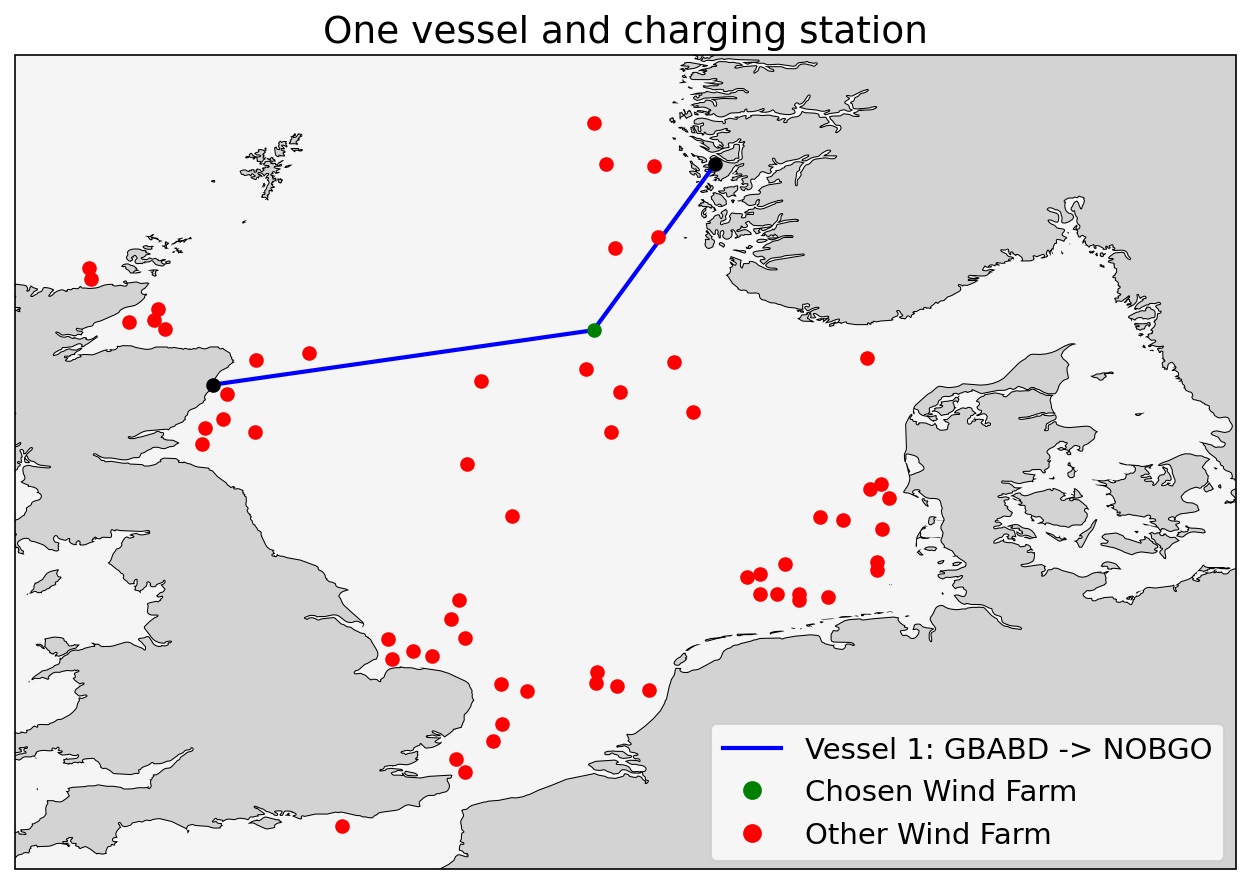
\includegraphics[width=\textwidth]{ch_facility_location/fig4_1a_route_scenario1.png}
  \par\smallskip{\small (a) Sailing route Scenario 1.}
\end{minipage}\hfill
\begin{minipage}[b]{0.48\textwidth}
  \centering
  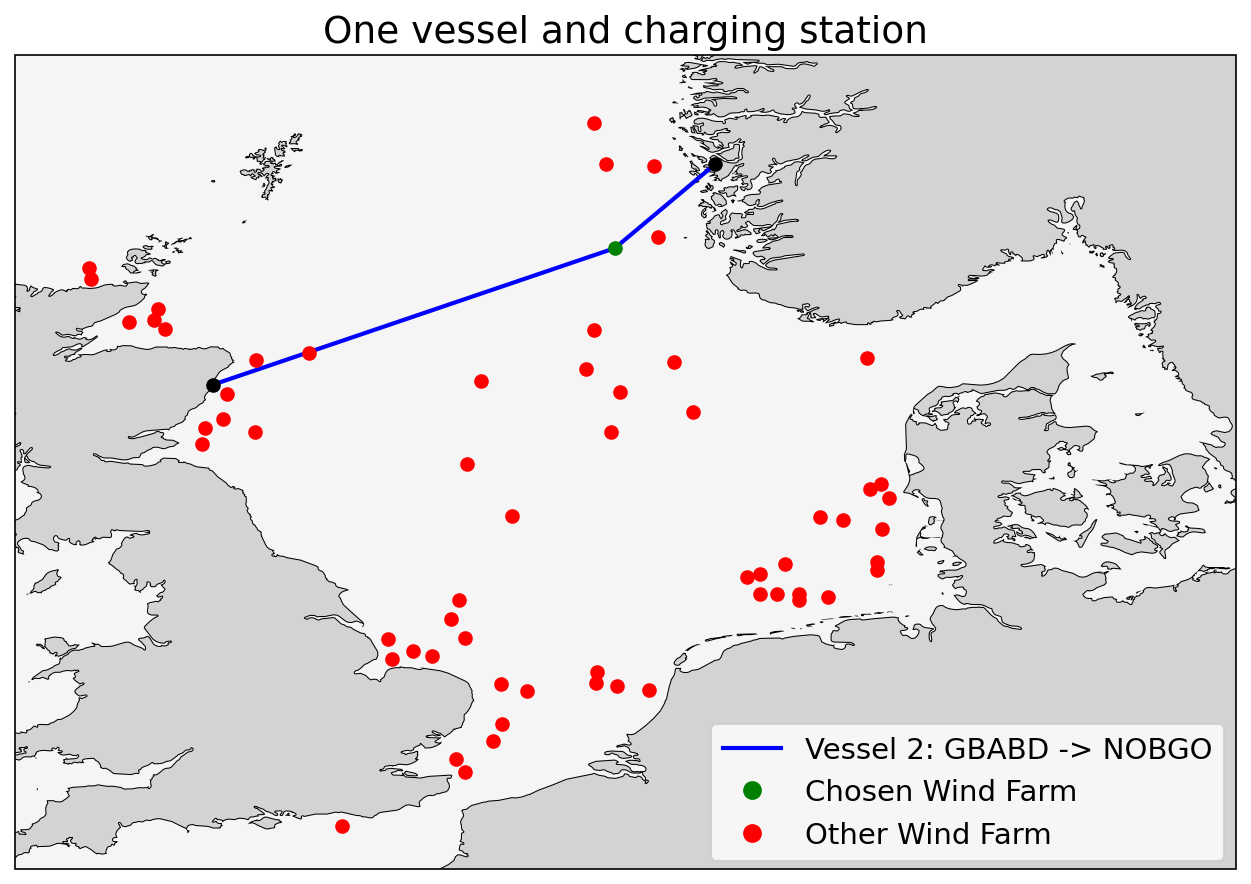
\includegraphics[width=\textwidth]{ch_facility_location/fig4_1b_route_scenario2.png}
  \par\smallskip{\small (b) Sailing route Scenario 2.}
\end{minipage}
\caption{Sailing routes.}
\label{fig:single-routes}
\end{figure}

\begin{figure}[H]
\centering
\begin{minipage}[b]{0.48\textwidth}
  \centering
  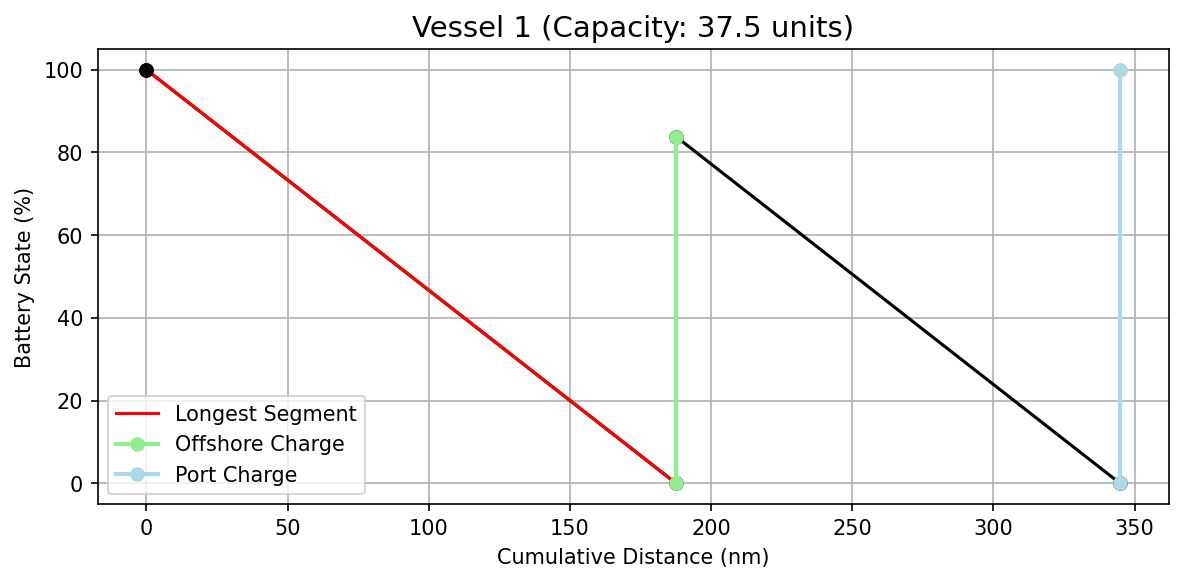
\includegraphics[width=\textwidth]{ch_facility_location/fig4_2a_soc_scenario1.png}
  \par\smallskip{\small (a) Scenario 1.}
\end{minipage}\hfill
\begin{minipage}[b]{0.48\textwidth}
  \centering
  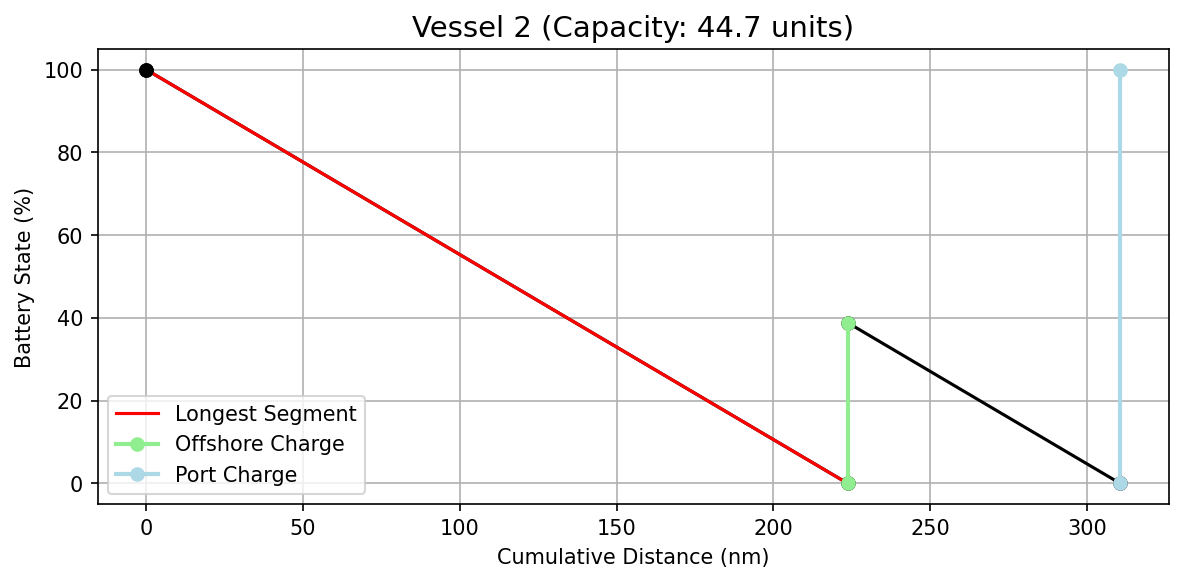
\includegraphics[width=\textwidth]{ch_facility_location/fig4_2b_soc_scenario2.png}
  \par\smallskip{\small (b) Scenario 2.}
\end{minipage}
\caption{SOC during voyage.}
\label{fig:single-soc}
\end{figure}

\subsubsection{Result consideration}
\label{sec:single-consideration}

The different outcomes from Scenario 1 and Scenario 2 demonstrate the model's core function of balancing competing costs to determine an optimal infrastructure placement. The selection of the single offshore charging station is as expected, dependent on the relative weighting between lost opportunity cost and sailing cost. When battery capacity has a high implicit cost (Scenario 1), the model prioritizes solutions that minimize the required battery size. This is achieved by selecting a charging station near the route's midpoint (\emph{Sørvest A}), thereby reducing the length of the longest segment between charges to 188 nm. This choice is made at the expense of deviating further from the most direct path. In contrast, when sailing distance represents the dominant cost (Scenario 2), the model favors a station placement (\emph{Vestavind E}) that facilitates a shorter overall voyage, accepting the need for a larger battery to cover the longer 224 nm leg as the more economical trade-off. This illustrates the link between optimal infrastructure location and the specific operational cost structure of the vessel.

\subsubsection{Charging strategies}
\label{sec:charging-strategies}

The model formulation, particularly through energy balance constraints (\ref{eq:energy-lo})--(\ref{eq:energy-hi}), currently allow the optimization model to determine the ideal amount of energy $x_{i}$ to recharge at each node. Under this strategy, the vessel might only partially recharge if it has enough energy for the next leg and completing the charge later is more cost-effective, considering energy prices.

This logic can be exemplified by a basic three-node route with an origin port as node 1, an offshore charging station as node 2, and a destination port as node 3. The amount of energy charged at the offshore station then depends on two factors: the relative energy prices offshore versus in port, and whether the first or last segment of the voyage is the longest. Figure~\ref{fig:charging-strategies} illustrates two scenarios, one where the distance from node 1 to 2 ($D_{12}$) is longest, and another where the distance from node 2 to 3 ($D_{23}$) is longest. Table~\ref{tab:charging-strategies} indicates the amount of energy charged offshore for each scenario assuming that the vessel leaves node 1 fully charged.

\begin{figure}[H]
\centering
\begin{minipage}[b]{0.48\textwidth}
  \centering
  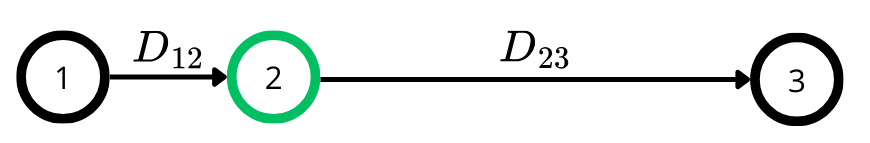
\includegraphics[width=\textwidth]{ch_facility_location/fig4_3a_D23_longest.png}
  \caption{Scenario where $D_{23}$ is longest.}
\end{minipage}\hfill
\begin{minipage}[b]{0.48\textwidth}
  \centering
  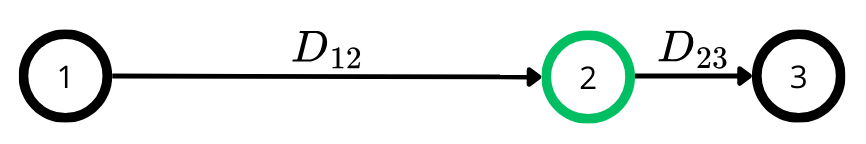
\includegraphics[width=\textwidth]{ch_facility_location/fig4_3b_D12_longest.png}
  \caption{Scenario where $D_{12}$ is longest.}
\end{minipage}
\caption{Charging strategy scenarios.}
\label{fig:charging-strategies}
\end{figure}

\begin{table}[H]
\centering
\caption{Energy charged at offshore charging station assuming leaving node 1 fully charged.}
\label{tab:charging-strategies}
\begin{tabular}{@{}l|c|c@{}}
\toprule
 & $C^{E}$ lowest in port & $C^{E}$ lowest offshore \\
\midrule
Segment $D_{12}$ longest & $E^{C}\cdot D_{23}$ & $E^{C}\cdot D_{12}$ \\
Segment $D_{23}$ longest & $E^{C}\cdot D_{12}$ & $E^{C}\cdot D_{12}$ \\
\bottomrule
\end{tabular}
\end{table}

While this flexibility allows for finding a potentially lower-cost solution, it increases the model's computational complexity. To assess the value of this flexibility and establish a simpler baseline for comparison, an alternative strategy enforces a mandatory full recharge at every node the vessel visits. This simplification is implemented by replacing the original constraints (\ref{eq:soc-le-q}) with more restrictive constraints, that forces the battery to be fully charged when departing any given node:

\begin{equation}
b_{i} \;=\; q \qquad \forall\, i\in\mathcal{W}
\label{eq:forced-full}
\end{equation}

\subsubsection{Illustrative case with forced full recharge}
\label{sec:forced-full-case}

To evaluate the impact of the 'forced full recharge' strategy, the two scenarios were re-optimized with constraints (\ref{eq:forced-full}) instead of (\ref{eq:soc-le-q}). Under this revised charging strategy, the optimization model ensures that the vessel begins its journey with fully charged batteries, and recharges the batteries completely at the offshore charging station and at the end of the journey. The results are summarized in Table~\ref{tab:forced-results}, with differences from the flexible charging outcomes noted in parentheses.

\begin{table}[H]
\centering
\caption{Forced full recharge results for Scenario 1 and Scenario 2 with differences compared to flexible charging in parentheses.}
\label{tab:forced-results}
\begin{tabular}{@{}lcc@{}}
\toprule
 & \textbf{Scenario 1} & \textbf{Scenario 2} \\
\midrule
Route                            & GBABD $\rightarrow$ NOBGO & GBABD $\rightarrow$ NOBGO \\
Charging station                 & Sørvest A & Peterhead (Vestavind E) \\
\textbf{Vessel-specific cost}    & \textbf{7733 ($+30$)} & \textbf{8931 ($+83$)} \\
\quad -- Sailing cost            & 3448 & 6074 ($-139$) \\
\quad -- Lost opportunity cost   & 3752 & 2500 ($+263$) \\
\quad -- Energy cost             & 532 ($+30$) & 357 ($-41$) \\
\quad -- Time cost               & 0 & 0 \\
\textbf{Total time in hours}     & \textbf{55.5} & \textbf{50.6 ($-1.2$)} \\
\quad -- Sailing                 & 23.0 & 20.3 ($-0.4$) \\
\quad -- Charging in port        & 15.7 ($-3.1$) & 25.0 ($+2.6$) \\
\quad -- Charging offshore       & 18.8 ($+3.1$) & 5.3 ($-3.4$) \\
Installed battery capacity $q_{v}$ & 37.5 & 50 ($+5.3$) \\
Total distance in nm             & 345 & 304 ($-7$) \\
\% of direct distance            & 114\% & 100\% ($-3\%$) \\
Longest segment in nm            & 188 & 250 ($+26$) \\
\bottomrule
\end{tabular}
\end{table}

\begin{figure}[H]
\centering
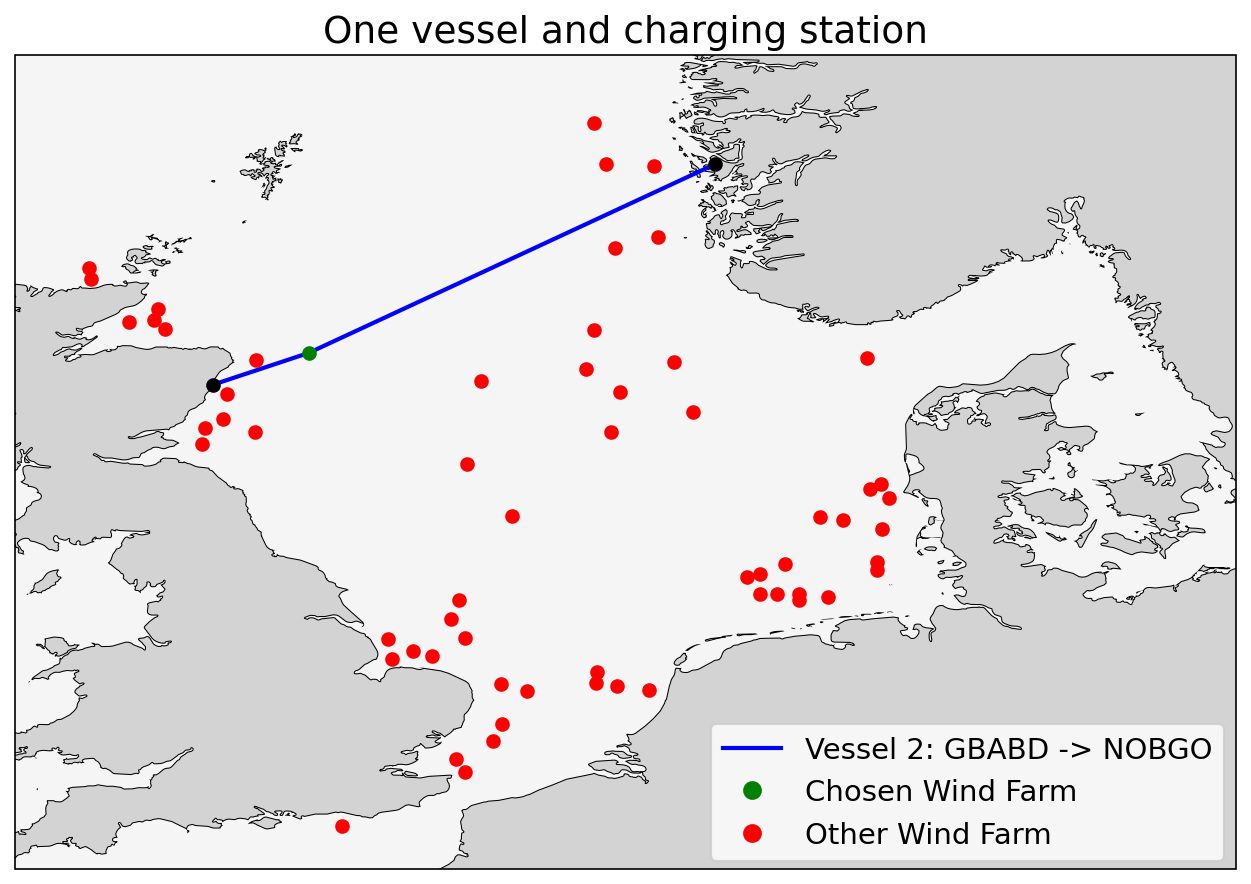
\includegraphics[width=0.62\textwidth]{ch_facility_location/fig4_4_route_forced_scenario2.png}
\caption{New sailing route for Scenario 2.}
\label{fig:forced-route}
\end{figure}

\begin{figure}[H]
\centering
\begin{minipage}[b]{0.48\textwidth}
  \centering
  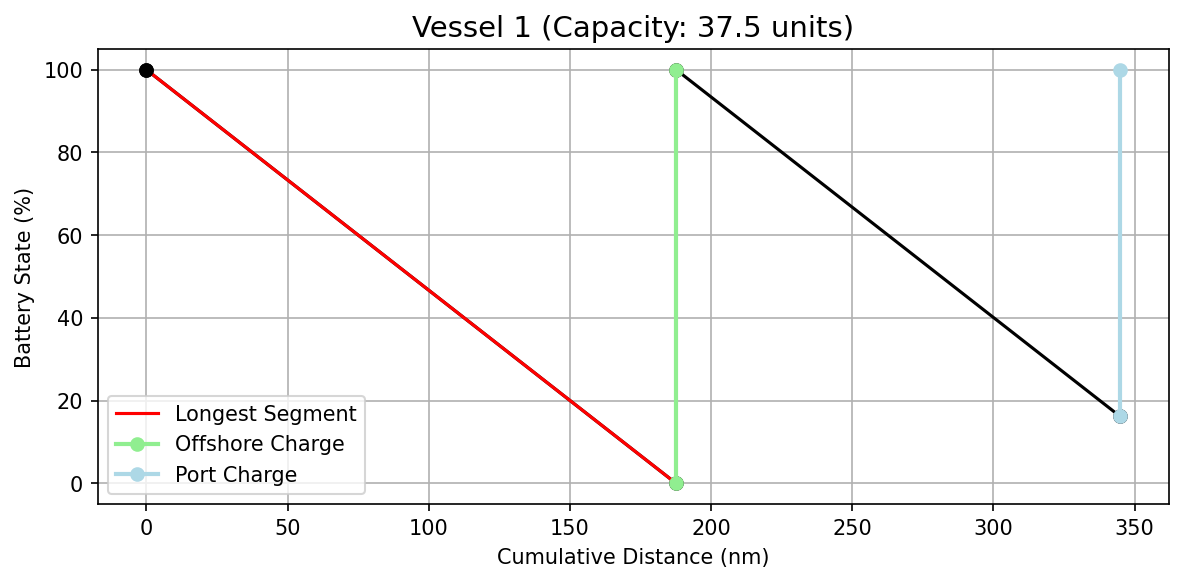
\includegraphics[width=\textwidth]{ch_facility_location/fig4_5a_soc_forced_scenario1.png}
  \par\smallskip{\small (a) Scenario 1.}
\end{minipage}\hfill
\begin{minipage}[b]{0.48\textwidth}
  \centering
  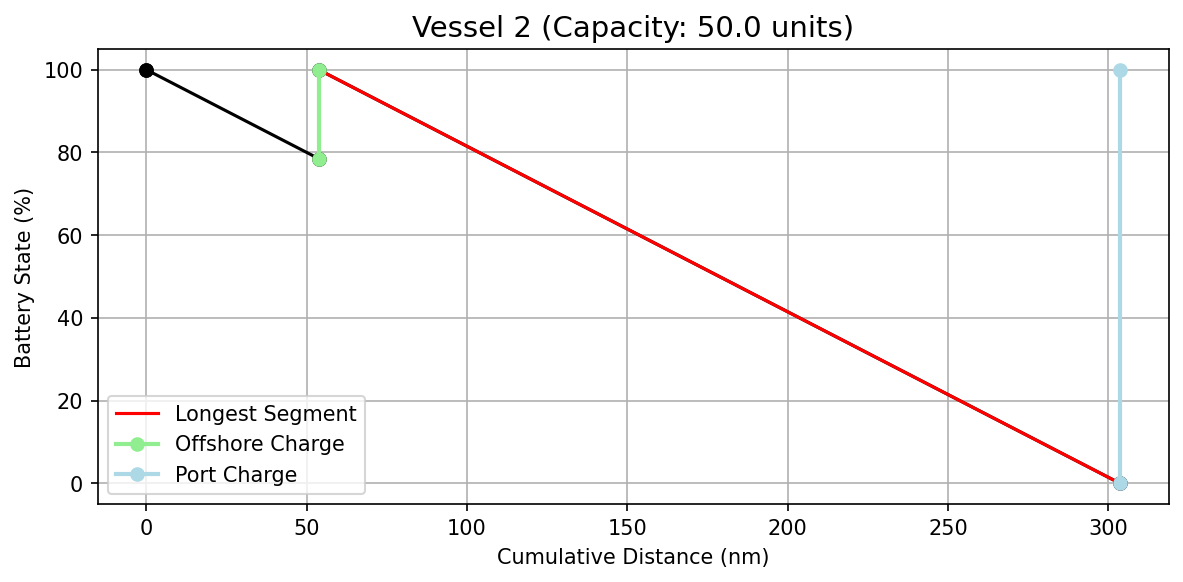
\includegraphics[width=\textwidth]{ch_facility_location/fig4_5b_soc_forced_scenario2.png}
  \par\smallskip{\small (b) Scenario 2.}
\end{minipage}
\caption{SOC with forced full charge at each node.}
\label{fig:forced-soc}
\end{figure}

In Scenario 1, forcing a full recharge did not alter the optimal route, charging station, or required battery capacity. The primary effects were a small increase in charging cost ($+30$) and a longer duration spent charging offshore ($+3.1$ hours), as the vessel now takes on more energy than strictly needed for the next leg. This can be seen when comparing Figure~\ref{fig:single-soc}a to Figure~\ref{fig:forced-soc}a.

However, in Scenario 2, enforcing a full recharge prompted a change in the optimal solution. Instead of Vestavind E, the model selected Peterhead (Figure~\ref{fig:forced-route}). This happens because fully recharging the larger battery required for the Vestavind E route would lead to a significant increase in charging costs for a relatively short final leg. The model, therefore, shifted the optimal station closer to the voyage's origin and increased battery capacity to accommodate a now longer final segment (Figure~\ref{fig:forced-soc}b). This shift demonstrates the model's adaptability to variations in operational charging strategies, a crucial consideration for robust real-world decision-making.

\subsubsection{General model simplifications}
\label{sec:single-simplifications}

This initial model iteration, while establishing a foundational structure, incorporates several simplifications. It does not account for operational uncertainties such as potential waiting times at charging stations, delays from adverse weather, or energy consumption variations due to sea state or vessel loading. Cost parameters, notably energy prices ($C^{E}_{i}$), are assumed static and uniform within location types (port vs.\ offshore), neglecting real-time volatility or site-specific costs. Energy consumption ($E^{C}$) is also simplified to a constant rate per nautical mile, disregarding factors like speed adjustments, currents, or wind. Lastly, the set of potential charging locations ($\mathcal{W}$) is fixed and predetermined, rather than allowing for dynamic placement.




\subsection{One vessel, one station}
\label{sec:fl-single}

\begin{figure}[htbp]
\centering
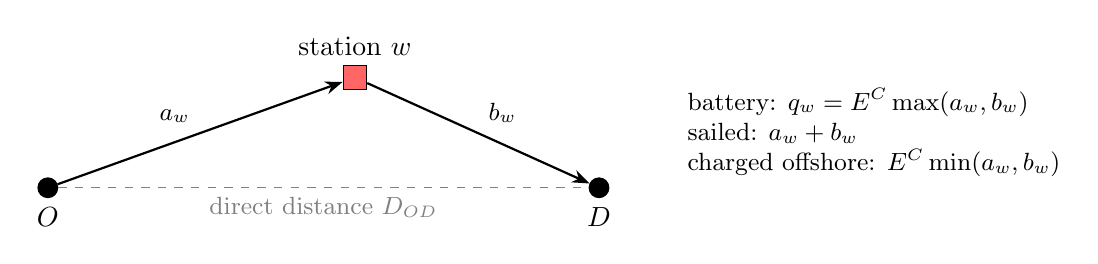
\begin{tikzpicture}[>={Stealth[length=2.2mm]},
  port/.style={circle,draw,fill=black,minimum size=2.5mm,inner sep=0pt},
  st/.style={rectangle,draw,fill=red!60,minimum size=3mm,inner sep=0pt}]
  \node[port,label=below:{$O$}] (O) at (0,0) {};
  \node[port,label=below:{$D$}] (D) at (7,0) {};
  \node[st,label=above:{station $w$}] (w) at (3.9,1.4) {};
  \draw[->,thick] (O) -- node[above left,font=\small]{$a_w$} (w);
  \draw[->,thick] (w) -- node[above right,font=\small]{$b_w$} (D);
  \draw[dashed,gray] (O) -- node[below,font=\small]{direct distance $D_{OD}$} (D);
  \node[align=left,font=\small,anchor=west] at (8.0,0.7)
  {battery: $q_w=E^C\max(a_w,b_w)$\\ sailed: $a_w+b_w$\\ charged offshore: $E^C\min(a_w,b_w)$};
\end{tikzpicture}
\caption{A single vessel charging once at station $w$ between origin $O$ and destination $D$.}
\label{fig:fl-odw}
\end{figure}

Consider a vessel sailing from origin $O$ to destination $D$ via station $w$, with legs $a_w=D_{Ow}$ and $b_w=D_{wD}$ as in Figure~\ref{fig:fl-odw}. The vessel consumes $E^C$ energy units per nautical mile, sails at speed $V$ and charges at rate $R^C$. It departs $O$ with a full battery and recharges to full at $D$, ready for the next voyage. Four cost components enter \citep{Agersborg2025}: a distance-dependent sailing cost $C^S$ per nautical mile; the energy cost, with price $C^E_p$ in port and $C^E_w$ offshore; a lost-opportunity cost $C^{LO}$ per unit of installed battery capacity, reflecting the cargo space the batteries occupy; and a time cost $C^T$ per hour of sailing and charging.

The battery capacity must be sufficient for the longest of the two legs, $q_w=E^C\max(a_w,b_w)$. When offshore energy is more expensive than port energy, the vessel charges only what it needs offshore, which is exactly $E^C\min(a_w,b_w)$ in both cases $a_w\ge b_w$ and $a_w<b_w$, and takes the remaining $E^C\max(a_w,b_w)$ in port. Total energy charged equals total consumption $E^C(a_w+b_w)$. Collecting terms, the cost of serving the vessel through station $w$ is
\begin{equation}
  c_w \;=\; \kappa\,(a_w+b_w) \;+\; C^{LO}E^C\max(a_w,b_w) \;+\; (C^E_w-C^E_p)\,E^C\min(a_w,b_w),
  \label{eq:fl-cw}
\end{equation}
with
\begin{equation*}
  \kappa \;=\; C^S + C^E_p E^C + C^T\left(\frac{1}{V}+\frac{E^C}{R^C}\right),
\end{equation*}
the cost per nautical mile sailed, including the port price of the energy consumed and the time spent both sailing and charging.

Equation \eqref{eq:fl-cw} reveals the structure of the problem. The first term is proportional to the total distance and is minimised by a station on or near the direct route; it is a \emph{median-type} term. The second term depends on the longest leg and is minimised by a station at the midpoint of the route; it is a \emph{center-type} (minimax) term. The third term penalises energy bought offshore and pulls the station towards one of the ports, where the shorter leg, and thus the offshore top-up, becomes small. The optimal station balances these three forces, and their relative weights are set by the vessel's cost structure.

\citet{Agersborg2025} analyses the route from Aberdeen to Bergen, whose direct distance is 302\,nm, with $E^C=0.2$, $C^E_w=10$, $C^E_p=5$ and $C^T=0$ in two scenarios. In Scenario~1, cargo space is valuable relative to sailing ($C^{LO}=100$, $C^S=10$), so \eqref{eq:fl-cw} becomes $c_w=11(a_w+b_w)+20\max(a_w,b_w)+\min(a_w,b_w)$, and the center-type term dominates. In Scenario~2, sailing is expensive relative to cargo space ($C^{LO}=50$, $C^S=20$), so $c_w=21(a_w+b_w)+10\max(a_w,b_w)+\min(a_w,b_w)$, and the median-type term dominates. Since there is only one station to choose, the problem is solved by evaluating \eqref{eq:fl-cw} for all 62 candidates and picking the cheapest. Table~\ref{tab:fl-single} shows the best candidates.

\begin{table}[htbp]
\centering
\caption{Best single charging stations for the Aberdeen--Bergen route. Legs and distances in nm, battery capacity $q_w$ in energy units, costs in monetary units. Bold entries mark the optimum in each scenario.}
\label{tab:fl-single}
\small
\begin{tabular}{@{}lrrrrrr@{}}
\toprule
Station $w$ & $a_w$ & $b_w$ & $a_w+b_w$ & $q_w$ & $c_w$ Scenario 1 & $c_w$ Scenario 2 \\
\midrule
S{\o}rvest A      & 188 & 157 & 345 & 37.5 & \textbf{7\,703} & 9\,275 \\
Vestavind E       & 224 &  87 & 311 & 44.7 & 7\,978 & \textbf{8\,848} \\
S{\o}rvest B      & 180 & 191 & 371 & 38.2 & 8\,075 & 9\,873 \\
Culzean           & 129 & 220 & 350 & 44.1 & 8\,382 & 9\,674 \\
Peterhead         &  54 & 250 & 304 & 50.0 & 8\,393 & 8\,931 \\
\bottomrule
\end{tabular}
\end{table}

In Scenario~1 the optimum is S{\o}rvest A, close to the midpoint, which keeps the battery small at the price of a route 14\,\% longer than the direct one. In Scenario~2 the optimum is Vestavind E, close to Bergen, which gives an almost direct route but a battery almost 20\,\% larger. Both costs agree with the full mixed-integer model in the thesis, which is a useful check: the closed-form expression \eqref{eq:fl-cw} captures everything the larger model does for this simple case. Note also S{\o}rvest B, which splits the route most evenly but still needs a slightly larger battery than S{\o}rvest A and adds a longer detour: balanced legs are not the same as a short longest leg.

\subsection{A fleet sharing one station}
\label{sec:fl-fleet}

Now let a set $\mathcal{V}$ of vessels, each with its own route and cost parameters, share a single station. Computing $c_{vw}$ from \eqref{eq:fl-cw} for every vessel $v$ and candidate $w$, the problem becomes
\begin{equation}
  \min_{w\in\mathcal{W}}\ \sum_{v\in\mathcal{V}} c_{vw},
  \label{eq:fl-1median}
\end{equation}
which is a 1-median problem in which each vessel plays the role of a customer and $c_{vw}$ the role of the assignment cost. What looked like a routing problem has become a classical location problem once the cost of each vessel--station combination is computed in advance.

For the four-vessel fleet in \citet{Agersborg2025}, the optimum is S{\o}rvest D, with a total cost of 41\,309, identical to the thesis result. The individual vessels fare very differently. Vessels 2 and 3 pay what they would pay with their own best station, whereas Vessel~1, sailing from Bergen to Aberdeen, pays 9\,889 instead of 7\,703 and sails a route 46\,\% longer than the direct one. A shared station is a compromise, and the compromise falls unevenly. If the station is financed jointly, this raises a question the optimisation model cannot answer: how should the cost be shared among vessels that benefit very differently?

There is one more observation to make. The thesis requires every vessel to call at the station. If Vessel~1 were instead allowed to sail directly with a battery large enough for the whole crossing, its cost would be 9\,376, which is lower than 9\,889. Allowing the ``no station'' option reduces the total to 40\,796 while S{\o}rvest D remains optimal. Whether a do-nothing alternative is included is a modelling choice with real consequences, and it is also exactly what is needed to measure the value of the infrastructure.

\subsection{A fleet with several stations}
\label{sec:fl-multi}

With several stations, a vessel may charge more than once. Let a \emph{charging plan} $k$ be a feasible sequence of stops for one vessel, for instance ``direct'', ``via S{\o}rvest A'' or ``via S{\o}rvest A, then Dogger Bank A\&B''. For each vessel we enumerate a set of plans $\mathcal{K}_v$, and for each plan we compute its cost $c_{vk}$ and record the set of stations $\mathcal{W}_k$ it uses. The cost of a multi-stop plan follows the same logic as \eqref{eq:fl-cw}: the battery covers the longest leg, and at each offshore stop the vessel charges just enough to reach the next stop. With binary $y_w=1$ if a station is built at $w$, and $z_{vk}=1$ if vessel $v$ uses plan $k$, the problem is
\begin{align}
  \min\quad & \sum_{v\in\mathcal{V}}\sum_{k\in\mathcal{K}_v} c_{vk}\, z_{vk} \label{eq:fl-plan-obj}\\
  \text{s.t.}\quad & \sum_{k\in\mathcal{K}_v} z_{vk} = 1 && \forall v\in\mathcal{V}, \label{eq:fl-plan-one}\\
  & z_{vk} \le y_w && \forall v\in\mathcal{V},\ k\in\mathcal{K}_v,\ w\in\mathcal{W}_k, \label{eq:fl-plan-open}\\
  & \sum_{w\in\mathcal{W}} y_w \le S^{\max}, \label{eq:fl-plan-S}\\
  & z_{vk}\ge 0,\; y_w\in\{0,1\}. \nonumber
\end{align}
Compare this with the $p$-median problem \eqref{eq:fl-pmed-obj}--\eqref{eq:fl-pmed-p}. Vessels take the place of customers, plans the place of assignments, \eqref{eq:fl-plan-one} is the assignment constraint, and \eqref{eq:fl-plan-open} is the strong ``open to use'' constraint, now required for every station a plan relies on. This is the path-based formulation of the flow refuelling location model \citep{Kuby2005}. Replacing \eqref{eq:fl-plan-S} by a fixed cost $\sum_w f_w y_w$ in the objective gives the corresponding UFLP.

With 62 candidates and at most two stops, each vessel has $1+62+62\cdot 61=3\,845$ plans, or 15\,380 for the fleet. Most are useless: a two-stop plan that costs more than a one-stop plan through one of its own stations can never be selected, and neither can a plan that costs more than sailing directly. Removing such dominated plans leaves 587 plans, and the model solves in a couple of seconds even with an open-source solver. With $S^{\max}=4$ the optimum builds stations at Dogger Bank A\&B, S{\o}rvest A, S{\o}rlige Nordsj{\o} II and Deutsche Bucht, at a total cost of 32\,952. Vessel~1 now charges once at S{\o}rvest A, its individual optimum, while the three other vessels charge twice. Stations, plans and vessel costs coincide with the thesis results, obtained there with a considerably larger arc-based formulation (Section~\ref{sec:fl-arc}); the reported totals differ by one unit due to rounding.

\begin{figure}[htbp]
\centering
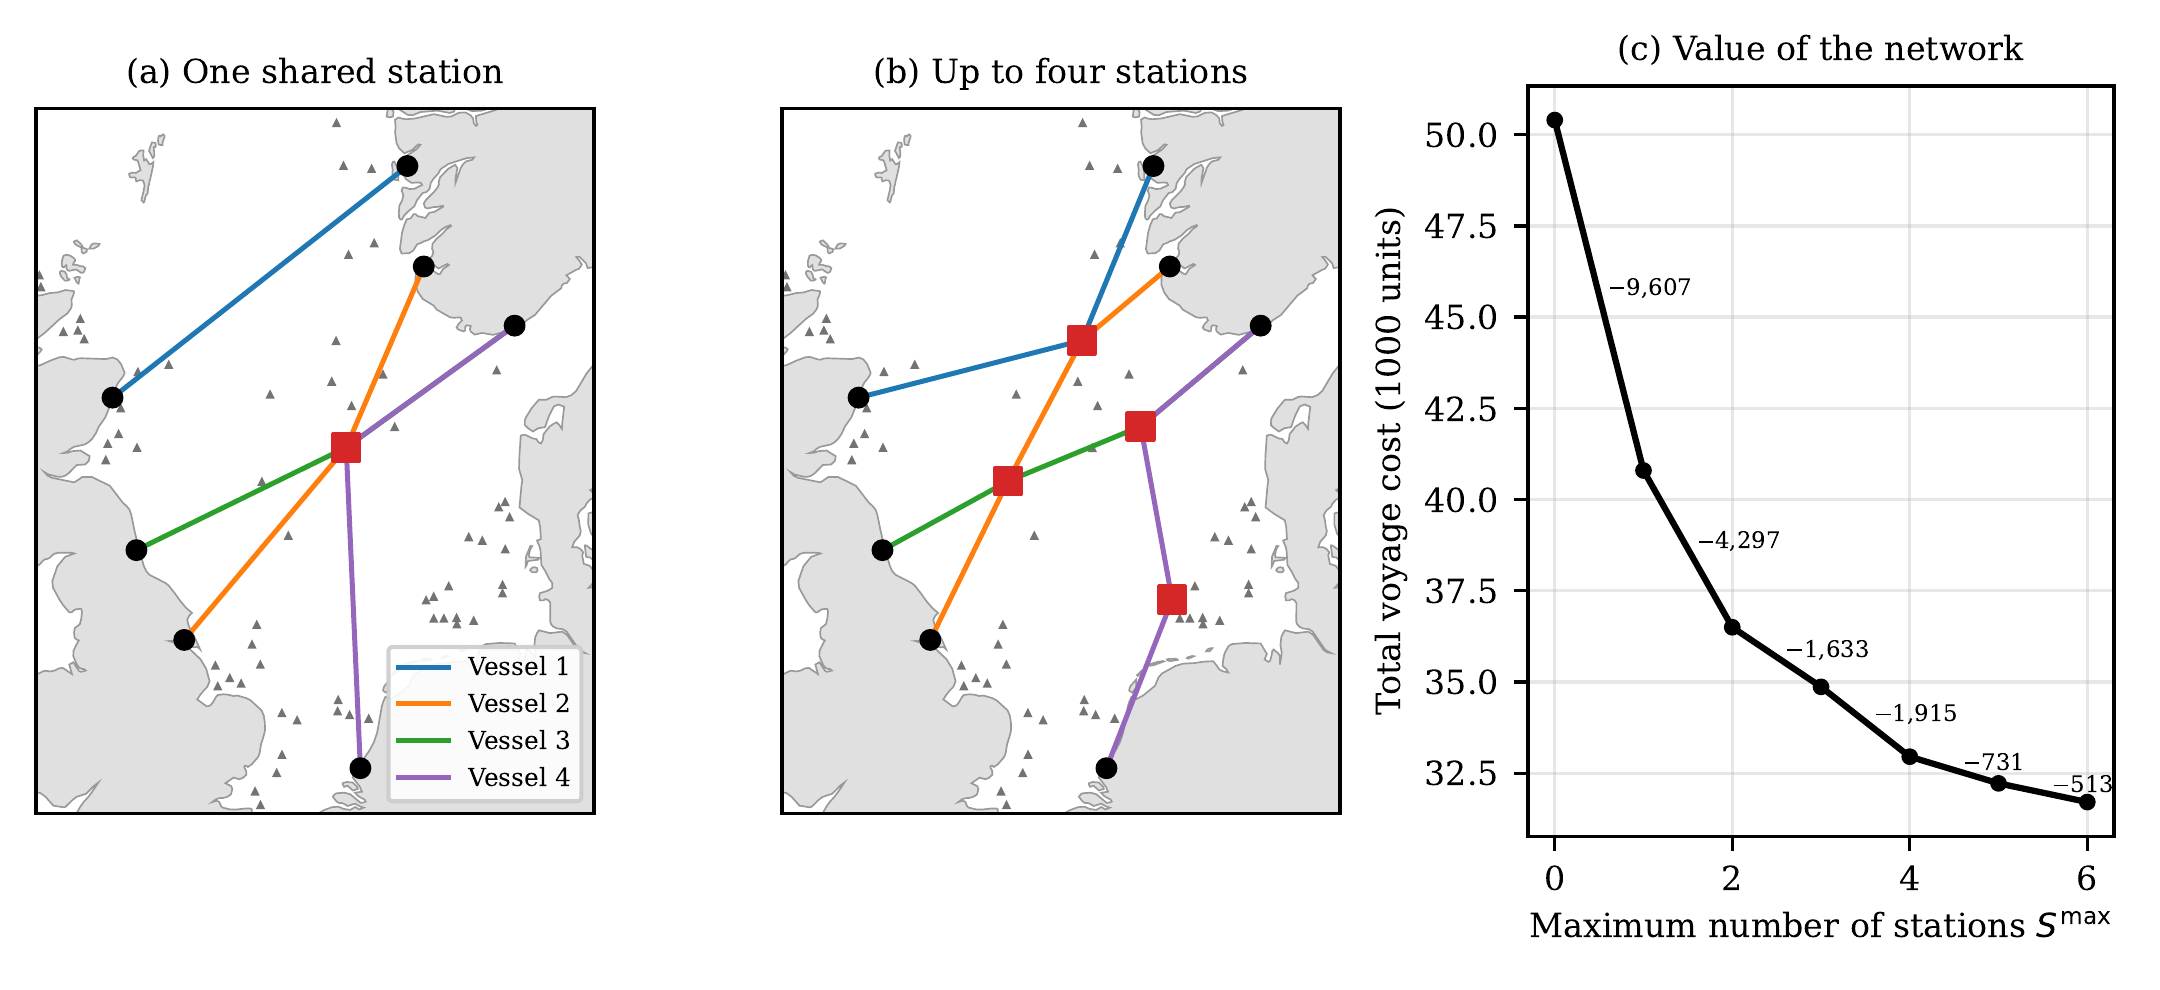
\includegraphics[width=\textwidth]{ch_facility_location/fl_charging_network.png}
\caption{Offshore charging for the four-vessel fleet. (a) One shared station at S{\o}rvest D; Vessel~1 sails directly. (b) Four stations. Grey triangles are the candidate wind farms, red squares the selected stations. (c) Minimum total voyage cost as a function of the maximum number of stations, with the saving from each additional station.}
\label{fig:fl-charging}
\end{figure}

Solving the model for $S^{\max}=0,1,\dots,6$ traces the \emph{value of the network}, shown in Figure~\ref{fig:fl-charging}(c). The first station reduces the fleet's cost by 9\,607, the second by 4\,297, the third by 1\,633, the fourth by 1\,915, and the fifth and sixth by 731 and 513. Two features deserve attention. First, the optimal configurations are not nested: the best pair of stations (S{\o}rvest C and Dogger Bank C) contains neither the best single station (S{\o}rvest D) nor any of the stations in the best set of four. Second, the marginal value of a station is not monotonically decreasing, as the fourth station is worth more than the third. Both features are consequences of the combinatorial nature of the problem, where the value of a station depends on which other stations it can be combined with. For an infrastructure developer who builds stations one at a time, this means that the first investment should be chosen with the final network in mind, a point we return to when we study decisions under uncertainty.

The curve also indicates how much a station must cost before it is no longer worth building. If the fixed cost per station, expressed per the same accounting period as the voyage costs, exceeds the marginal saving, the station should not be built. The thesis develops this idea into an estimate of the price premium shipowners would be willing to pay for offshore energy \citep{Agersborg2025}.

\subsection{The integrated arc-based formulation}
\label{sec:fl-arc}

The plan-based formulation is transparent and fast, but it relies on two simplifications: every relevant plan must be enumerated, and the cost of each plan must be computable in advance. Both break down when vessels call at many ports in sequence, when the number of stops per leg grows, or when the charging amount at each stop is itself a decision with a non-trivial trade-off. \citet{Agersborg2025} therefore formulates the problem directly on the network of ports and candidate stations. For a single vessel, let $z_{ij}=1$ if the vessel sails arc $(i,j)$, $b_i$ the battery level when departing node $i$, $x_i$ the energy charged at node $i$ and $q$ the installed capacity. The core of the model is
\begin{align}
  \min\quad & \sum_{(i,j)\in\mathcal{A}} C^S D_{ij} z_{ij} + \sum_{i\in\mathcal{N}} C^E_i x_i + C^{LO} q + C^T\Big(\sum_{(i,j)\in\mathcal{A}}\frac{D_{ij}}{V}z_{ij} + \sum_{i\in\mathcal{N}}\frac{x_i}{R^C}\Big) \label{eq:fl-arc-obj}\\
  \text{s.t.}\quad & \text{flow conservation \eqref{eq:fl-flowcons} with one unit from $O$ to $D$ on the variables } z_{ij}, \nonumber\\
  & b_j \ge b_i - E^C D_{ij} + x_j - M(1-z_{ij}) && \forall (i,j)\in\mathcal{A}, \label{eq:fl-arc-b1}\\
  & b_j \le b_i - E^C D_{ij} + x_j + M(1-z_{ij}) && \forall (i,j)\in\mathcal{A}, \label{eq:fl-arc-b2}\\
  & b_i \ge E^C D_{ij} - M(1-z_{ij}) && \forall (i,j)\in\mathcal{A}, \label{eq:fl-arc-b3}\\
  & b_i \le q, \quad b_O = b_D = q, \quad q\le Q, \label{eq:fl-arc-q}\\
  & \sum_{k:(k,w)\in\mathcal{A}} z_{kw} \le y_w \quad \forall w\in\mathcal{W}, \qquad \sum_{w\in\mathcal{W}} y_w \le S^{\max}. \label{eq:fl-arc-y}
\end{align}
The flow conservation constraints route the vessel, and constraints \eqref{eq:fl-arc-b1}--\eqref{eq:fl-arc-b2} are the energy balance along the arcs actually sailed: if $z_{ij}=1$, the battery level on departing $j$ equals the level on departing $i$, minus the consumption on the leg, plus what is charged at $j$. If $z_{ij}=0$, the big-$M$ terms deactivate the constraints. Constraint \eqref{eq:fl-arc-b3} ensures that the vessel has enough energy for every leg it sails, and \eqref{eq:fl-arc-y} links the route to the station decisions exactly as in the location models. For a fleet, all routing and energy variables receive a vessel index $v$, while $y_w$ remains common.

Two technical points are worth making. First, $M$ must be derived from the bounds on the quantities in the constraints, for example $M\ge Q+E^C\max_{(i,j)}D_{ij}$, and should be no larger than necessary, for the reasons discussed in Section~\ref{sec:fl-strength}. A value tied to the number of nodes, which is natural in the ordering constraints below, does not in general bound energy terms. Second, when a vessel may visit several stations, the routing variables can form \emph{subtours}, disconnected cycles among station nodes that satisfy flow conservation without being part of the voyage. These must be eliminated, for instance with the Miller--Tucker--Zemlin ordering constraints \citep{Miller1960} or the Dantzig--Fulkerson--Johnson cut-set constraints \citep{Dantzig1954}. Subtours and their elimination are a central topic in routing, and we return to them in a later chapter.

The arc-based model is a genuine \emph{location--routing--sizing} model: it decides where to build infrastructure, how each vessel sails, how much it charges where, and how large its battery must be, all at once. The plan-based model solves the same problem for the instances in this chapter because the routing and charging sub-problem of each vessel is simple enough to be solved in advance by enumeration. That two very different formulations yield the same optimum is also a valuable check on both implementations.

\subsection{What the model leaves out}
\label{sec:fl-limits}

The charging models in this section minimise the operating cost of the fleet and treat the infrastructure as free up to the limit $S^{\max}$. In reality, an offshore station requires substantial investment, and it will usually be built and operated by someone other than the shipowners who use it. A complete analysis therefore has at least two decision makers: an infrastructure provider who chooses locations and prices to recover its investment, and shipowners who choose routes, charging plans and battery sizes in response. Such leader--follower structures lead to bilevel optimisation problems, which lie beyond the scope of this course, but the value-of-network curve in Figure~\ref{fig:fl-charging}(c) is a first step towards them.

Other simplifications are shared with the bunkering hub example. Stations and hubs are assumed to have unlimited power or throughput, so queuing at popular stations is ignored. Energy consumption is assumed constant per nautical mile, independent of weather, sea state and loading. And all parameters, from energy prices and freight rates to the fleet that will actually adopt battery-electric propulsion, are treated as known. For infrastructure with a lifetime of decades, that last assumption is the most problematic, and handling it properly is the subject of the chapter on decisions under uncertainty.


% ---------------------------------------------------------------------
\section{Summary and outlook}
\label{sec:fl-summary}

Facility location problems are network design problems in which the decision is which nodes to establish. The classical models differ mainly in their objective. Covering models express service standards, median models express efficiency, center models express worst-case service, and fixed-charge models let the number of facilities follow from the trade-off between investment and operating cost. As the bunkering hub example showed, the choice of objective can change the solution completely, and making that choice consciously is part of the design task.

On the modelling side, three lessons carry over to integer programming in general. Formulations with the same integer solutions can differ greatly in the strength of their LP relaxation, and the disaggregated ``open to use'' constraint $x_{ij}\le y_i$ is the standard example. A complex problem can sometimes be turned into a classical one by computing assignment costs in advance, as we did when each vessel's charging plan was reduced to a cost and a set of required stations. And the optimal configurations of combinatorial problems need not be nested or show diminishing returns, which has real consequences for how infrastructure is rolled out over time.

In the next chapter we take the network as given and ask how to use it efficiently. The shortest path problem finds the best route through a network, for instance the sailing route between two ports via a set of waypoints, and the maximum flow problem determines how much a network can carry, for instance the throughput capacity of a port or a supply chain. Both are network flow problems in the sense of Section~\ref{sec:fl-networks}, and both have the remarkable property that their LP relaxations have integer optimal solutions, so no branching is needed at all.


\backmatter
\bibliographystyle{plainnat}
\bibliography{compendium}

\end{document}
